 %% ++++++++++++++++++++++++++++++++++++++++++++++++++++++++++++
%% Hauptdatei, Wurzel des Dokuments
%% ++++++++++++++++++++++++++++++++++++++++++++++++++++++++++++
%
%  Gerüst:
%  * Version 0.13
%  * M.Sc. Silvia Krug, silvia.krug@tu-ilmenau.de
%  * Fachgebiet Kommunikationsnetze, TU Ilmenau
%  Modifiziert von:
%  * Eric Gorkow Januar 2020
%
%  Für Hauptseminare, Studienarbeiten, Diplomarbeiten
%
%  Autor           : Eric Gorkow
%  Letzte Änderung : Morgen
%

% Headerfeld, Typ des Dokumentes, einzubindende Packages.
% Hier bei Bedarf Änderungen vornehmen.

% only change this if you know what you do
%  Gerüst:
%  * Version 1.0
%  * B.Eng. Eric Gorkow
%  * Student, TU Ilmenau
%  * Januar 2020
%
%  Für Hauptseminare, Studienarbeiten, Diplomarbeiten
%
%  Autor           : Max Mustermann
%  Letzte Änderung : Morgen
%
\documentclass
[   twoside=false,     % Einseitiger oder zweiseitiger Druck?
fontsize=12pt,     % Bezug: 12-Punkt Schriftgröße
DIV=15,            % Randaufteilung, siehe Dokumentation "KOMA"-Script
BCOR=0mm,         % Bindekorrektur: Innen 17mm Platz lassen. Copyshop-getestet.
%    headsepline,
headsepline,  % Unter Kopfzeile Trennlinie (aus: headnosepline)
footsepline,  % Über Fußzeile Trennlinie (aus: footnosepline)
open=right,        % Neue Kapitel im zweiseitigen Druck rechts beginnen lassen
paper=a4,          % Seitenformat A4
abstract=true,     % Abstract einbinden
listof=totoc,      % Div. Verzeichnisse ins Inhaltsverzeichnis aufnehmen
bibliography=totoc,% Literaturverzeichnis ins Inhaltsverzeichnis aufnehmen
titlepage,         % Titelseite aktivieren
headinclude=true,  % Seiten-Head in die Satzspiegelberechnung mit einbeziehen
footinclude=false, % Seiten-Foot nicht in die Satzspiegelberechnung mit einbeziehen
numbers=noenddot   % Gliederungsnummern ohne abschließenden Punkt darstellen
]   {scrreprt}         % Dokumentenstil: "Report" aus dem KOMA-Skript-Paket
\usepackage[table]{xcolor} % Anpassung tooltip
\usepackage[active]{srcltx}
%\usepackage[activate=normal]{pdfcprot} % Optischer Randausgleich -> pdflatex!
\usepackage{ifthen}
\usepackage[ngerman]{babel}   % Neue Deutsche Rechtschreibung
%\usepackage[latin1]{inputenc} % Zeichencodierung nach ISO-8859-1
\usepackage[utf8]{inputenc}   %	Zeichencodierung nach UTF-8 (Unicode)
\usepackage[T1]{fontenc}
\usepackage{lmodern} %Schriftart Latim modern
\usepackage[T1]{url}
\usepackage[final]{graphicx}
\usepackage[automark]{scrlayer-scrpage}
\usepackage{setspace}
%\usepackage[first,light]{draftcopy} % Für Probedruck
\usepackage{tabularx}
\usepackage{tikz}

\usepackage[plainpages=false,pdfpagelabels,hypertexnames=false]{hyperref}

%%% Modifications
\setlength{\parindent}{0em}%Einrücken der ersten Zeile eines neuen Absatz 0=keiner
\usepackage{float}
\usepackage[section]{placeins}
\usepackage{pdfpages}
\restylefloat{figure}
\usepackage[printonlyused,nohyperlinks]{acronym} % Anpassung
\usepackage{amsmath} % Anpassung
\usepackage{pdfcomment}% Anpassung tooltip
\usepackage{listings}
\lstset{numbers=left,stepnumber=2,, numberstyle=\tiny, numbersep=5pt, basicstyle=\small,}
% used Language
\lstset{language=Matlab}
\usepackage{hyperxmp} % metadata addon

%%% Matlab2tikz
\usepackage{pgfplots}
\pgfplotsset{compat=newest}
%% the following commands are needed for some matlab2tikz features
\usetikzlibrary{plotmarks}
\usetikzlibrary{arrows, arrows.meta, shapes.geometric}
\usepgfplotslibrary{patchplots}
\usepackage{grffile}
\usepackage{subfig}

\usepackage{attachfile} 

\tikzset{
	font={\upshape\selectfont}}
\newcommand\tikzmark[2][]{
	\tikz[remember picture,baseline=(#1.base),align=left]{\node[minimum width=\hsize](#1){$#2$};}
}

% Tiefe der Kapitelnummerierung beeinflussen
\setcounter{secnumdepth}{3} % Tiefe der Nummerierung
\setcounter{tocdepth}{2}    % Tiefe des Inhaltsverzeichnisses

\usepackage[normalem]{ulem}
\newcommand{\markup}[1]{\textbf{#1}}

% Seitenlayout festlegen. Hier nichts ändern!
\pagestyle{scrplain}
\ihead[]{\headmark}
\ohead[]{\pagemark}
\chead[]{}
\ifoot[]{}
\ofoot[]{\scriptsize \artderausarbeitung\ \namedesautors}
\cfoot[]{}
\renewcommand{\titlepagestyle}{scrheadings}
\renewcommand{\partpagestyle}{scrheadings}
\renewcommand{\chapterpagestyle}{scrheadings}
\renewcommand{\indexpagestyle}{scrheadings}

% Abschnittsweise Nummerierung anstatt fortlaufend. Hier nichts ändern!
\makeatletter
\@addtoreset{equation}{chapter}
\@addtoreset{figure}{chapter}
\@addtoreset{table}{chapter}
\renewcommand\theequation{\thechapter.\@arabic\c@equation}
\renewcommand\thefigure{\thechapter.\@arabic\c@figure}
\renewcommand\thetable{\thechapter.\@arabic\c@table}
\makeatother

% Quelltextrahmen, klein. Hier nichts ändern!
\newsavebox{\inhaltkl}
\def\rahmenkl{\sbox{\inhaltkl}\bgroup\small\renewcommand{\baselinestretch}{1}\vbox\bgroup\hsize\textwidth}
\def\endrahmenkl{\par\vskip-\lastskip\egroup\egroup\fboxsep3mm%
	\framebox[\textwidth][l]{\usebox{\inhaltkl}}}

% Quelltextrahmen, normale Groesse. Hier nichts ändern!
\newsavebox{\inhalt}
\def\rahmen{\sbox{\inhalt}\bgroup\renewcommand{\baselinestretch}{1}\vbox\bgroup\hsize\textwidth}
\def\endrahmen{\par\vskip-\lastskip\egroup\egroup\fboxsep3mm%
	\framebox[\textwidth][l]{\usebox{\inhalt}}}

% Sonstige Befehlsdefinitionen hier ablegen.
\newcommand{\entspricht}{\stackrel{\wedge}{=}}

% Tabellenspaltendefinitionen mit fester Breite --> somit Zeilenumbruch innerhalb einer Zelle möglich
% aus http://www.torsten-schuetze.de/tex/tabsatz-2004.pdf
\usepackage{array, booktabs}
\newcolumntype{f}{>{$}l<{$}}
\newcolumntype{n}{>{\raggedright}l}
\newcolumntype{N}{>{\scriptsize}l}
\newcolumntype{v}[1]{>{\raggedright\hspace{0pt}}m{#1}}
\newcolumntype{V}[1]{>{\scriptsize\raggedright\hspace{0pt}}m{#1}}
\newcolumntype{Z}[1]{>{\raggedright\centering}m{#1}}
\newcolumntype{k}[1]{>{\raggedright}p{#1}}
% ergibt Tabllenspalte fester Breite, linksbündig
% Umbruch innerhalb der Zelle mit \\, neue Tabellezeile mit \tabularnewline
% \addlinespace für Gruppentrennung (aus \texttt{booktabs.sty})

% change this for individual style of table and flowchartstyle reasons
%  Gerüst:
%  * Version 1.0
%  * B.Eng. Eric Gorkow
%  * Student, TU Ilmenau
%  * Januar 2020
%
%  Für Hauptseminare, Studienarbeiten, Diplomarbeiten
%
%  Autor           : Max Mustermann
%  Letzte Änderung : Morgen
%

% own defines for table
\definecolor{headrowcolor}{RGB}{190, 190, 190}
\definecolor{lightrowcolor}{RGB}{217, 217, 217}

% own global flowchartsymbols
\tikzstyle{rect_round} =  [rectangle, rounded corners, minimum height = 1cm, text centered, text width=3.2cm, draw=black, fill=green!30]
\tikzstyle{rect_round_o} =  [rectangle, rounded corners, minimum height = 1cm, text centered, text width=3.2cm, draw=black, fill=orange!30]
\tikzstyle{rect_sharp} =  [rectangle, minimum height = 1cm, text centered, text width=3.2cm, draw=black, fill=blue!30]
\tikzstyle{influence} =  [rectangle,  minimum width=1cm, minimum height = 0.5cm]
\tikzstyle{oval_b} =  [ellipse, minimum height = 1cm, text centered, text width=3.2cm, draw=black, fill=blue!10]
\tikzstyle{oval_g} =  [ellipse, minimum height = 1cm, text centered, draw=black, fill=gray!10]

\tikzstyle{arrow} = [thick,->,>=stealth]
\tikzstyle{line} = [thick,-]

% own colors for diagranms
\definecolor{tuilmenau}{RGB}{0, 102, 102}
\definecolor{efshell}{RGB}{142,19,88}
\definecolor{efsdunkel}{RGB}{86,8,56}
\definecolor{efsrot}{RGB}{229,47,64}
\definecolor{efsdunkelblau}{RGB}{0,115,173}
\definecolor{efshellblau}{RGB}{0,152,169}
\definecolor{efsgrün}{RGB}{92,167,75}
\definecolor{efsgelb}{RGB}{241,132,24}

\colorlet{balkenpositiv1}{efshellblau}
\colorlet{balkenpositiv2}{efsgrün}

\colorlet{balkennegativ1}{efsgelb}
\colorlet{balkennegativ2}{efsrot}

\colorlet{plotpositiv1}{efsgrün}
\colorlet{plotpositiv2}{efshell}

\colorlet{plotnegativ1}{efsdunkelblau}
\colorlet{plotnegativ2}{efsrot}

% replacing colors of pictures via \colorlet{mycolor1}{plotpositiv1} within the picture%



% Hier in die zweite geschweifte Klammer jeweils
% die persönlichen Daten und das Thema der Arbeit eintragen:
\newcommand{\artderausarbeitung}{Musterarbeit}
\newcommand{\namedesautors}{Max Mustermann}
\newcommand{\themaderarbeit}{Titel der Arbeit}
\newcommand{\jahrderabgabe}{2020}
\newcommand{\monatderabgabe}{01}
\newcommand{\tagderabgabe}{01}

% Was ist ein Abstract? 
% Ein kurze, prägnante Aussage/Zusammen über den Inhalt der Arbeit. Wird unteranderem zur Katalogisierung für Bibliografien genutzt und wird zu diesem Zweck auf der Artikelsprache und in Englisch verfasst.
\newcommand{\abstractger}{Deutsche Version 50-100 Wörter}
\newcommand{\abstracteng}{Englische Version 50-100 Wörter}

% PDF Metadaten definieren
\hypersetup{
	pdftitle={\themaderarbeit},
	pdfauthor={\namedesautors},
	pdfkeywords={\artderausarbeitung; TU-Ilmenau; Prozessoptimierung;}, % Weitere Stichwörter hinzufürgen!
	pdfdate={\jahrderabgabe-\monatderabgabe-\tagderabgabe},
	pdftype={\artderausarbeitung},
	pdfsubject={\abstracteng},% auf wunsch ändern, für Bibliografie ist Englisch aber immer sinnvoller
}

% Trennvorschläge für falsch getrennte Wörter.
% Wird häufig bei eingedeutschen Wörtern benötigt, da LaTeX hierbei
% gerne falsch trennt. Alternativ kann auch im Fliesstext ein
% Trennvorschlag per "\-" hinterlegt werden, bspw.:
% Die Hard\-ware besteht aus A und B.
\hyphenation{
	Hard-ware
}

%%% Modifications own commands
% tooltip modification
% to use reference put the glsc.cwl in AppData\Roaming\texstudio\completion\user (if file is lost the create one with equivalent name and wirte '/glsc{label}#r' into it)
%restart TexStudio
% after that go to 'Configurate TexStudio' (tab Options) and select the Completement Tab. Check the new file in that list and its done. 
\newcommand*{\glsc}[1]{\pdftooltip{\gls*{#1}}{\glsentrydesc{#1}}}
% achtung funktioniert nur mit nohyperlinks im usepackage des acronym paketes, * zum unterdrücken hier leider nicht wirksam
\renewcommand*{\ac}[1]{\pdftooltip{\acs{#1}}{\acl{#1}}}
% da die Funktion von \ac, dass beim ersten Aufruf die lange UND Kurze version abgebildet wird durch die redefinition abgeschaltet ist
% bei erster Nutzung wird daher dieser Befehle benötigt
\newcommand*{\acfirst}[1]{\pdftooltip{\acf{#1}}{\acl{#1}}}

\usepackage[
nonumberlist, %keine Seitenzahlen anzeigen
toc,          %Einträge im Inhaltsverzeichnis
section=chapter]      %im Inhaltsverzeichnis auf section-Ebene erscheinen
{glossaries}[=v4.49]
\usepackage{hyperref}

\newglossary[slg]{symbolslist}{syi}{syg}{Symbolverzeichnis}
\renewcommand*{\glspostdescription}{}
\makeglossaries

%Eigener Gloassarystyle
\newglossarystyle{MyStyle}{
  \glossarystyle{long3colheader}
  \renewenvironment{theglossary}
  {\begin{longtable}{lp{2cm}p{\glsdescwidth}}}
    {\end{longtable}}
  \renewcommand*{\glossaryheader}{\textbf{Symbol} & \textbf{Einheit} &
    \textbf{Beschreibung}\\[3ex]\endhead}% ÄNDERUNG: Kopf auf jeder Seite wiederholen
  \renewcommand*{\glossaryentryfield}[5]{%
    \glsentryitem{##1}\glstarget{##1}{##2} & ##4 & ##3  \\[1ex]}%
}
%%% Beispiel!!
    % Aufruf folgendermaßen :
    % \gls{symb:phiy}
\newglossaryentry{symb:phiy}{
name={\ensuremath{\varphi_{y}}},
symbol={Grad},
description={Winkel der Kugel in y-Richtung},
sort=symbolphiy, 
type=symbolslist}

%%% Begin der Aufzählung
\newglossaryentry{symb:m}{
	name={m},
	symbol={kg},
	description={Masse},
	sort=symbolm,
	type=symbolslist}

\newglossaryentry{symb:mdot}{
	name={\ensuremath{\dot{m}}},
	symbol={kg/s)},
	description={Massenstrom},
	sort=symbolmdot,
	type=symbolslist}

\newglossaryentry{symb:mdot_Luft}{
	name={\ensuremath{\dot{m}\textsubscript{Luft}}},
	symbol={kg/s)},
	description={Massenstrom Luft},
	sort=symbolmdotLuft,
	type=symbolslist}

\newglossaryentry{symb:m_Cell}{
	name={m\textsubscript{Cell}},
	symbol={kg},
	description={Masse},
	sort=symbolm\_cell,
	type=symbolslist}

\newglossaryentry{symb:v}{
	name={v},
	symbol={m/s},
	description={Geschwindigkeit},
	sort=symbolv,
	type=symbolslist}

\newglossaryentry{symb:v_Luft}{
	name={v\textsubscript{Luft}},
	symbol={m/s},
	description={Luft Geschwindigkeit},
	sort=symbolvLuft,
	type=symbolslist}

\newglossaryentry{symb:E_kin}{
	name={E\textsubscript{kin}},
	symbol={J},
	description={Kinetische Energie},
	sort=symbolE\_kin,
	type=symbolslist}

\newglossaryentry{symb:mu}{
	name={\ensuremath{\mu}},
	symbol={-},
	description={Effizienz},
	sort=symbolmu,
	type=symbolslist}

\newglossaryentry{symb:I_cell}{
	name={I\textsubscript{cell}},
	symbol={A},
	description={Zellstrom},
	sort=symbolI\_cell,
	type=symbolslist}

\newglossaryentry{symb:R_cell}{
	name={R\textsubscript{cell}},
	symbol={\ensuremath{Omega}},
	description={Innerer Wiederstand einer Zelle},
	sort=symbolR\_cell,
	type=symbolslist}

\newglossaryentry{symb:G_th}{
	name={G\textsubscript{th}},
	symbol={W/K},
	description={thermischer Leitwert einer Zelle},
	sort=symbolG\_th,
	type=symbolslist}

\newglossaryentry{symb:T_celli}{
	name={T\textsubscript{cell i}},
	symbol={K},
	description={Zelltemperatur am Punkt i},
	sort=symbolT\_celli,
	type=symbolslist}

\newglossaryentry{symb:T_celli+1}{
	name={T\textsubscript{cell i+1}},
	symbol={K},
	description={Zelltemperatur am Punkt i+1},
	sort=symbolT\_celli+1,
	type=symbolslist}

\newglossaryentry{symb:T_u}{
	name={T\textsubscript{u}},
	symbol={K},
	description={Umgebungstemperatur},
	sort=symbolT\_u,
	type=symbolslist}

\newglossaryentry{symb:G_r}{
	name={G\textsubscript{r}},
	symbol={\ensuremath{m^2}},
	description={Strahlungsfaktor},
	sort=symbolG\_r,
	type=symbolslist}

\newglossaryentry{symb:SBoltz}{
	name={\ensuremath{\sigma}},
	symbol={\ensuremath{W/(m^2K^4)}},
	description={Stefan Boltzmann Konstante},
	sort=symbolSBoltz,
	type=symbolslist}

\newglossaryentry{symb:C_B}{
	name={C\textsubscript{Cell}},
	symbol={\ensuremath{J/K}},
	description={kapazität einer Zelle},
	sort=symbolC\_B,
	type=symbolslist}

\newglossaryentry{symb:A}{
	name={A},
	symbol={\ensuremath{m^2}},
	description={Fläche},
	sort=symbolA,
	type=symbolslist}

\newglossaryentry{symb:A_r}{
	name={A\textsubscript{r}},
	symbol={\ensuremath{m^2}},
	description={Fläche real},
	sort=symbolAr,
	type=symbolslist}

\newglossaryentry{symb:A_m}{
	name={A\textsubscript{m}},
	symbol={\ensuremath{m^2}},
	description={Fläche modell},
	sort=symbolAm,
	type=symbolslist}

\newglossaryentry{symb:Qdot}{
	name={\ensuremath{\dot{Q}}},
	symbol={\ensuremath{W}},
	description={Wärmestrom},
	sort=symbolQdot,
	type=symbolslist}

\newglossaryentry{symb:Qdot_r}{
	name={\ensuremath{\dot{Q}}\textsubscript{r}},
	symbol={\ensuremath{W}},
	description={Wärmestrom real},
	sort=symbolQdotr,
	type=symbolslist}

\newglossaryentry{symb:Qdot_m}{
	name={\ensuremath{\dot{Q}}\textsubscript{m}},
	symbol={\ensuremath{W}},
	description={Wärmestrom modell},
	sort=symbolQdotm,
	type=symbolslist}

\newglossaryentry{symb:P_Luft}{
	name={\ensuremath{P}\textsubscript{Luft}},
	symbol={\ensuremath{W}},
	description={Luftleistung},
	sort=symbolPLuft,
	type=symbolslist}

\newglossaryentry{symb:P_elektrisch}{
	name={\ensuremath{P}\textsubscript{elektrisch}},
	symbol={\ensuremath{W}},
	description={Elektrische Leistung},
	sort=symbolPelektrisch,
	type=symbolslist}

\newglossaryentry{symb:deltaT_ein r}{
	name={\ensuremath{\Delta}T\textsubscript{ein r}},
	symbol={\ensuremath{K}},
	description={reale temperaturdifferenz am Eingang},
	sort=symboldeltaTeinr,
	type=symbolslist}

\newglossaryentry{symb:t_ein Wasser}{
	name={t\textsubscript{ein Wasser}},
	symbol={\ensuremath{°C}},
	description={Wassereintrittstemperatur},
	sort=symbolteinwasser,
	type=symbolslist}

\newglossaryentry{symb:t_aus Wasser}{
	name={t\textsubscript{aus Wasser}},
	symbol={\ensuremath{°C}},
	description={Wasseraustrittstemperatur},
	sort=symboltauswasser,
	type=symbolslist}

\newglossaryentry{symb:deltaT_ein m}{
	name={\ensuremath{\Delta}T\textsubscript{ein m}},
	symbol={\ensuremath{K}},
	description={modell temperaturdifferenz am Eingang},
	sort=symboldeltaTeinm,
	type=symbolslist}

\newglossaryentry{symb:Cv_wasser}{
	name={C\textsubscript{v Wasser}},
	symbol={\ensuremath{J/KgK}},
	description={Isochore Wärmekapazität Wasser},
	sort=symbolCvwasser,
	type=symbolslist}

\newglossaryentry{symb:Vdot_wasser}{
	name={\ensuremath{\dot{V}\textsubscript{Wasser}}},
	symbol={\ensuremath{Kg/s}},
	description={Volumenstrom Wasser},
	sort=symbolVdotwasser,
	type=symbolslist}

\newglossaryentry{symb:Vdot_Luft}{
	name={\ensuremath{\dot{V}\textsubscript{Luft}}},
	symbol={\ensuremath{Kg/s}},
	description={Volumenstrom Luft},
	sort=symbolVdotLuft,
	type=symbolslist}

\newglossaryentry{symb:rho_wasser}{
	name={\ensuremath{\rho}\textsubscript{Wasser}},
	symbol={\ensuremath{Kg/m^3}},
	description={Dichte Wasser},
	sort=symbolrhowasser,
	type=symbolslist}

\newglossaryentry{symb:rho_Luft}{
	name={\ensuremath{\rho}\textsubscript{Luft}},
	symbol={\ensuremath{Kg/m^3}},
	description={Dichte Luft},
	sort=symbolLuft,
	type=symbolslist}

\newglossaryentry{symb:F}{
	name={F},
	symbol={\ensuremath{N}},
	description={Kraft},
	sort=symbolkraft,
	type=symbolslist}

\newglossaryentry{symb:F_Schub}{
	name={F\textsubscript{Schub}},
	symbol={\ensuremath{N}},
	description={Schubkraft},
	sort=symbolSchubkraft,
	type=symbolslist}

\newglossaryentry{symb:A_Prop}{
	name={A\textsubscript{Prop}},
	symbol={\ensuremath{m^2}},
	description={Propellerfläche},
	sort=symbolPropellerfläche,
	type=symbolslist}

\newglossaryentry{symb:eta_Luefter}{
	name={\ensuremath{\eta}\textsubscript{Luefter}},
	symbol={\ensuremath{-}},
	description={Lüftereffizienz},
	sort=symboletaLuefter,
	type=symbolslist}

\newglossaryentry{symb:U_H}{
	name={U\textsubscript{H}},
	symbol={\ensuremath{V}},
	description={Obere Hysteresespannung},
	sort=symbolUH,
	type=symbolslist}

\newglossaryentry{symb:U_L}{
	name={U\textsubscript{L}},
	symbol={\ensuremath{V}},
	description={Untere Hysteresespannung},
	sort=symbolUL,
	type=symbolslist}

\newglossaryentry{symb:U_HA}{
	name={U\textsubscript{HA}},
	symbol={\ensuremath{V}},
	description={Oberer Spannungspegel},
	sort=symbolUHA,
	type=symbolslist}

\newglossaryentry{symb:U_LA}{
	name={U\textsubscript{LA}},
	symbol={\ensuremath{V}},
	description={Unterer Spannungspegel},
	sort=symbolULA,
	type=symbolslist}

\newglossaryentry{symb:U_ref}{
	name={U\textsubscript{ref}},
	symbol={\ensuremath{V}},
	description={Referenzspannung},
	sort=symbolUref,
	type=symbolslist}

\newglossaryentry{symb:VCC}{
	name={VCC},
	symbol={\ensuremath{V}},
	description={Voltage Controlled Current (meißt Versorgungsspannung)},
	sort=symbolVCC,
	type=symbolslist}

\newglossaryentry{symb:U_a}{
	name={U\textsubscript{a}},
	symbol={\ensuremath{V}},
	description={Ausgangsspannung},
	sort=symbolUa,
	type=symbolslist}

\newglossaryentry{symb:U_e}{
	name={U\textsubscript{e}},
	symbol={\ensuremath{V}},
	description={Eingangsspannung},
	sort=symbolUe,
	type=symbolslist}

\newglossaryentry{symb:R}{
	name={R},
	symbol={\ensuremath{\omega}},
	description={Wiederstand},
	sort=symbolR,
	type=symbolslist}

\newglossaryentry{symb:C}{
	name={C},
	symbol={F},
	description={Kapazität},
	sort=symbolC,
	type=symbolslist}

\newglossaryentry{symb:t}{
	name={t},
	symbol={s},
	description={Zeit in sekunden},
	sort=symbolt,
	type=symbolslist}

\newglossaryentry{symb:e}{
	name={e},
	symbol={-},
	description={Euler Zahl},
	sort=symbole,
	type=symbolslist}

\newglossaryentry{symb:tau}{
	name={\ensuremath{\tau}},
	symbol={s},
	description={Zeitkonstante},
	sort=symboltau,
	type=symbolslist}

\newglossaryentry{symb:I}{
	name={\ensuremath{I}},
	symbol={A},
	description={Strom},
	sort=symbolI,
	type=symbolslist}

\newglossaryentry{symb:U}{
	name={\ensuremath{U}},
	symbol={V},
	description={Spannung},
	sort=symbolU,
	type=symbolslist}

\newglossaryentry{symb:K}{
	name={\ensuremath{K}},
	symbol={-},
	description={Anwendungsfaktor},
	sort=symbolK,
	type=symbolslist}

\newglossaryentry{symb:T_SW}{
	name={\ensuremath{T\textsubscript{SW}}},
	symbol={°C},
	description={Schalttemperatur},
	sort=symbolTSW,
	type=symbolslist}

\newglossaryentry{symb:C_th}{
	name={\ensuremath{C\textsubscript{th}}},
	symbol={J/K},
	description={Wärmekapazität},
	sort=symbolCTH,
	type=symbolslist}

\newglossaryentry{symb:N_PTC}{
	name={\ensuremath{N\textsubscript{PTC}}},
	symbol={-},
	description={Anzahl der PTC`s},
	sort=symbolNPTC,
	type=symbolslist}

\newglossaryentry{symb:N_dump}{
	name={\ensuremath{N\textsubscript{dump}}},
	symbol={-},
	description={Anzahl der Entladezyklen in folge},
	sort=symbolNdump,
	type=symbolslist}

\newglossaryentry{symb:V_out}{
	name={\ensuremath{U\textsubscript{out}}},
	symbol={V},
	description={Ausgangsspannung},
	sort=symbolVout,
	type=symbolslist}

\newglossaryentry{symb:V_inmax}{
	name={\ensuremath{U\textsubscript{in max}}},
	symbol={V},
	description={maximale Eingangsspannung},
	sort=symbolVinmax,
	type=symbolslist}

\newglossaryentry{symb:V_inmin}{
	name={\ensuremath{U\textsubscript{in min}}},
	symbol={V},
	description={minimale Eingangsspannung},
	sort=symbolVinmin,
	type=symbolslist}

\newglossaryentry{symb:NP/NS}{
	name={\ensuremath{NP/NS}},
	symbol={-},
	description={Primär- Sekundärwicklungsverhältnis des Transformators},
	sort=symbolNPNS,
	type=symbolslist}

\newglossaryentry{symb:NP/NS_ideal}{
	name={\ensuremath{NP/NS_ideal}},
	symbol={-},
	description={Ideales Primär- Sekundärwicklungsverhältnis des Transformators},
	sort=symbolNPNSideal,
	type=symbolslist}

\newglossaryentry{symb:NS/NP}{
	name={\ensuremath{NS/NP}},
	symbol={-},
	description={Sekundär- Primärwicklungsverhältnis des Transformators},
	sort=symbolNSNP,
	type=symbolslist}

\newglossaryentry{symb:D_min}{
	name={\ensuremath{D\textsubscript{min}}},
	symbol={-},
	description={Minimaler Duty Cycle},
	sort=symbolDmin,
	type=symbolslist}

\newglossaryentry{symb:D_max}{
	name={\ensuremath{D\textsubscript{max}}},
	symbol={-},
	description={Maximaler Duty Cycle},
	sort=symbolDmax,
	type=symbolslist}

\newglossaryentry{symb:T_blank}{
	name={\ensuremath{T\textsubscript{blank}}},
	symbol={ns},
	description={extended blanking time},
	sort=symbolTblank,
	type=symbolslist}

\newglossaryentry{symb:f_osc}{
	name={\ensuremath{f\textsubscript{osc}}},
	symbol={kHz},
	description={Taktfrequenz},
	sort=symbolTblank,
	type=symbolslist}

\newglossaryentry{symb:T_cycle}{
	name={\ensuremath{T\textsubscript{cycle}}},
	symbol={ns},
	description={Zyklenzeit},
	sort=symbolTcycle,
	type=symbolslist}

\newglossaryentry{symb:OnTime_min}{
	name={\ensuremath{On Time\textsubscript{min}}},
	symbol={ns},
	description={Minimale eingeschaltete Zeit},
	sort=symbolOnTimemin,
	type=symbolslist}

\newglossaryentry{symb:T_Sense}{
	name={\ensuremath{T\textsubscript{Sense}}},
	symbol={ns},
	description={Strommesszeit},
	sort=symbolTSense,
	type=symbolslist}

\newglossaryentry{symb:I_Ripple}{
	name={\ensuremath{I\textsubscript{Ripple}}},
	symbol={A},
	description={Ripple Strom},
	sort=symbolIRipple,
	type=symbolslist}

\newglossaryentry{symb:V_Ripple}{
	name={\ensuremath{V\textsubscript{Ripple}}},
	symbol={A},
	description={Ripple Spannung},
	sort=symbolVRipple,
	type=symbolslist}

\newglossaryentry{symb:L_O}{
	name={\ensuremath{L\textsubscript{O}}},
	symbol={H},
	description={Ausgangsinduktivität},
	sort=symbolLO,
	type=symbolslist}

\newglossaryentry{symb:C_O}{
	name={\ensuremath{C\textsubscript{O}}},
	symbol={F},
	description={Ausgangskapazität},
	sort=symbolCO,
	type=symbolslist}

\newglossaryentry{symb:ESR}{
	name={\ensuremath{ESR}},
	symbol={\ensuremath{Omega}},
	description={Equivalenter Serieller Wiederstand},
	sort=symbolESR,
	type=symbolslist}

\newglossaryentry{symb:H_Prim}{
	name={\ensuremath{H\textsubscript{Prim}}},
	symbol={\ensuremath{H}},
	description={Primärinduktivität des Transformators},
	sort=symbolHPrim,
	type=symbolslist}

\newglossaryentry{symb:C_CL}{
	name={\ensuremath{C\textsubscript{CL}}},
	symbol={\ensuremath{F}},
	description={Kapazität des Clamp Kondensators},
	sort=symbolCCL,
	type=symbolslist}

\newglossaryentry{symb:C_S}{
	name={\ensuremath{C\textsubscript{S}}},
	symbol={\ensuremath{F}},
	description={Kapazität des Snubber Kondensators},
	sort=symbolCS,
	type=symbolslist}

\newglossaryentry{symb:R_S}{
	name={\ensuremath{R\textsubscript{S}}},
	symbol={\ensuremath{F}},
	description={Widerstand des Snubber Widerstandes},
	sort=symbolRS,
	type=symbolslist}

\newglossaryentry{symb:V_DS}{
	name={\ensuremath{V\textsubscript{DS}}},
	symbol={\ensuremath{V}},
	description={Spannung zwischen Drain und Source},
	sort=symbolVDS,
	type=symbolslist}

\newglossaryentry{symb:I_out}{
	name={\ensuremath{I\textsubscript{out}}},
	symbol={\ensuremath{A}},
	description={Ausgangsstrom},
	sort=symbolIout,
	type=symbolslist}

\newglossaryentry{symb:P_conduction}{
	name={\ensuremath{P\textsubscript{conduction}}},
	symbol={\ensuremath{W}},
	description={Leistung bei durchgeschaltetem Zustand},
	sort=symbolPconduction,
	type=symbolslist}

\newglossaryentry{symb:P_Gatedriver}{
	name={\ensuremath{P\textsubscript{Gatedriver}}},
	symbol={\ensuremath{W}},
	description={Leistung des Gatetreibers},
	sort=symbolPGatedriver,
	type=symbolslist}

\newglossaryentry{symb:P_Turn on}{
	name={\ensuremath{P\textsubscript{Turn on}}},
	symbol={\ensuremath{W}},
	description={Leistung im Einschaltzustand},
	sort=symbolPTurnon,
	type=symbolslist}

\newglossaryentry{symb:P_Turn off}{
	name={\ensuremath{P\textsubscript{Turn off}}},
	symbol={\ensuremath{W}},
	description={Leistung im Ausschaltzustand},
	sort=symbolPTurnoff,
	type=symbolslist}

\newglossaryentry{symb:P_gesamt}{
	name={\ensuremath{P\textsubscript{gesamt}}},
	symbol={\ensuremath{W}},
	description={Gesamtleistung},
	sort=symbolPgesamt,
	type=symbolslist}

\newglossaryentry{symb:R_DS on}{
	name={\ensuremath{R\textsubscript{DS on}}},
	symbol={\ensuremath{\Omega}},
	description={Leitwiederstand im durchgeschalteten Zustand},
	sort=symbolRDSon,
	type=symbolslist}

\newglossaryentry{symb:Q_G}{
	name={\ensuremath{Q\textsubscript{G}}},
	symbol={\ensuremath{C}},
	description={Gate Ladung},
	sort=symbolQG,
	type=symbolslist}

\newglossaryentry{symb:Q_GD}{
	name={\ensuremath{Q\textsubscript{GD}}},
	symbol={\ensuremath{C}},
	description={Gate zu Drain Ladung},
	sort=symbolQGD,
	type=symbolslist}

\newglossaryentry{symb:INTV_CC}{
	name={\ensuremath{INTV\textsubscript{CC}}},
	symbol={\ensuremath{V}},
	description={Interne Spannungsversorgung},
	sort=symbolINTVCC,
	type=symbolslist}

\newglossaryentry{symb:I_Gate}{
	name={\ensuremath{I\textsubscript{Gate}}},
	symbol={\ensuremath{A}},
	description={Gate Treiber Strom},
	sort=symbolIGate,
	type=symbolslist}

\newglossaryentry{symb:R_Akku}{
	name={\ensuremath{R\textsubscript{Akku}}},
	symbol={\ensuremath{\Omega}},
	description={Innenwiederstand des Akkus},
	sort=symbolRAkku,
	type=symbolslist}

\newglossaryentry{symb:N_Parallel}{
	name={\ensuremath{N\textsubscript{Parallel}}},
	symbol={\ensuremath{-}},
	description={Anzahl der Parallelen Akkuzellen},
	sort=symbolNParallel,
	type=symbolslist}

\newglossaryentry{symb:N_Seriell}{
	name={\ensuremath{N\textsubscript{Seriell}}},
	symbol={\ensuremath{-}},
	description={Anzahl der Seriellen Akuzellen},
	sort=symbolNSeriell,
	type=symbolslist}

\newglossaryentry{symb:U_Akku}{
	name={\ensuremath{U\textsubscript{Akku}}},
	symbol={\ensuremath{V}},
	description={Akkuspannung},
	sort=symbolUAkku,
	type=symbolslist}

\newglossaryentry{symb:U_cell}{
	name={\ensuremath{U\textsubscript{cell}}},
	symbol={\ensuremath{V}},
	description={Zellspannung},
	sort=symbolUCell,
	type=symbolslist}

\newglossaryentry{symb:I_Akku}{
	name={\ensuremath{I\textsubscript{Akku}}},
	symbol={\ensuremath{A}},
	description={Akku Kurzschlusstrom},
	sort=symbolIAkku,
	type=symbolslist}


\newglossaryentry{symb:kappa}{
	name={\ensuremath{\kappa}},
	symbol={1/m},
	description={Krümmung},
	sort=symbolkappa,
	type=symbolslist}
\newglossaryentry{symb:kappad}{
	name={\ensuremath{\dot{\kappa}}},
	symbol={1/(m*s)},
	description={Krümmungsänderung},
	sort=symbolkappad, 
	type=symbolslist}
\newglossaryentry{symb:s}{
	name={\ensuremath{s}},
	symbol={m},
	description={Lauflänge, Längsachse der Frenet-Koordinaten},
	sort=symbols, 
	type=symbolslist}
\newglossaryentry{symb:d}{
	name={\ensuremath{d}},
	symbol={m},
	description={Querversatz, Querachse der Frenet-Koordinaten},
	sort=symboldd, 
	type=symbolslist}
\newglossaryentry{symb:sd}{
	name={\ensuremath{\dot{s}}},
	symbol={m/s},
	description={1.Ableitung der Lauflänge},
	sort=symbolsd, 
	type=symbolslist}
\newglossaryentry{symb:dd}{
	name={\ensuremath{\dot{d}}},
	symbol={m/s},
	description={1.Ableitung des Querversatzes},
	sort=symboldd, 
	type=symbolslist}
\newglossaryentry{symb:sdd}{
	name={\ensuremath{\ddot{s}}},
	symbol={m/s},
	description={2.Ableitung der Lauflänge},
	sort=symbolsdd, 
	type=symbolslist}
\newglossaryentry{symb:ddd}{
	name={\ensuremath{\ddot{d}}},
	symbol={m/s},
	description={2.Ableitung des Querversatzes},
	sort=symbolddd, 
	type=symbolslist}
\newglossaryentry{symb:psi}{
	name={\ensuremath{\psi}},
	symbol={$^\circ$},
	description={Orientierung},
	sort=symbolpsi, 
	type=symbolslist}
\newglossaryentry{symb:psid}{
	name={\ensuremath{\dot{\psi}}},
	symbol={$^\circ$/s},
	description={Orientierungänderung},
	sort=symbolpsid, 
	type=symbolslist}
\newglossaryentry{symb:deltapsi}{
	name={\ensuremath{\Delta\psi}},
	symbol={$^\circ$},
	description={Differenz zu Referenzorientierung},
	sort=symboldeltapsi, 
	type=symbolslist}
\newglossaryentry{symb:deltapsid}{
	name={\ensuremath{\Delta\dot{\psi}}},
	symbol={$^\circ$/s},
	description={Änderung der Differenz zu Referenzorientierung},
	sort=symboldeltapsid, 
	type=symbolslist}
\newglossaryentry{symb:vd}{
	name={\ensuremath{\dot{v}}},
	symbol={m/$s^2$},
	description={Geschwindigkeitsänderung},
	sort=symbolvd, 
	type=symbolslist}
\newglossaryentry{symb:a}{
	name={\ensuremath{a}},
	symbol={m/$s^2$},
	description={Beschleunigung},
	sort=symbola, 
	type=symbolslist}
\newglossaryentry{symb:ad}{
	name={\ensuremath{\dot{a}}},
	symbol={m/$s^3$},
	description={Beschleunigungsänderung},
	sort=symbolad, 
	type=symbolslist}
\newglossaryentry{symb:aquer}{
	name={\ensuremath{a_{Quer}}},
	symbol={m/$s^2$},
	description={Querbeschleunigung},
	sort=symbolaquer, 
	type=symbolslist}
\newglossaryentry{symb:j}{
	name={\ensuremath{j}},
	symbol={m/$s^3$},
	description={Ruck},
	sort=symbolj, 
	type=symbolslist}
\newglossaryentry{symb:kappar}{
	name={\ensuremath{\kappa_{r}}},
	symbol={1/m},
	description={Referenzkrümmung},
	sort=symbolkappar, 
	type=symbolslist}
\newglossaryentry{symb:u}{
	name={\ensuremath{u}},
	symbol={-},
	description={Systemeingang},
	sort=symbolu, 
	type=symbolslist}
\newglossaryentry{symb:aplat}{
	name={\ensuremath{a_{plat}}},
	symbol={m/$s^2$},
	description={Beschleunigungsplateauwert des Längspolynoms},
	sort=symbolaplat, 
	type=symbolslist}
\newglossaryentry{symb:amaxl}{
	name={\ensuremath{a_{max längs}}},
	symbol={m/$s^2$},
	description={Maximaler Beschleunigungswert des Längspolynoms},
	sort=symbolamaxl, 
	type=symbolslist}
\newglossaryentry{symb:amaxd}{
	name={\ensuremath{a_{max quer}}},
	symbol={m/$s^2$},
	description={Maximaler Beschleunigungswert des Querpolynoms},
	sort=symbolamaxd, 
	type=symbolslist}
\newglossaryentry{symb:a0}{
	name={\ensuremath{a_{0}}},
	symbol={m/$s^2$},
	description={Startwert der Beschleunigung des Längspolynoms},
	sort=symbolanull, 
	type=symbolslist}
\newglossaryentry{symb:tau1}{
	name={\ensuremath{\tau_{1}}},
	symbol={s},
	description={Endzeitpunkt der ersten Ruckparabel des Längspolynoms},
	sort=symboltaul, 
	type=symbolslist}
\newglossaryentry{symb:tau2}{
	name={\ensuremath{\tau_{2}}},
	symbol={s},
	description={Anfangszeitpunkt der zweiten Ruckparabel des Längspolynoms},
	sort=symboltau2, 
	type=symbolslist}
\newglossaryentry{symb:tel}{
	name={\ensuremath{t_{e längs}}},
	symbol={s},
	description={Endzeitpunkt des Längspolynoms},
	sort=symboltel, 
	type=symbolslist}
\newglossaryentry{symb:v0}{
	name={\ensuremath{v_{0}}},
	symbol={m/s},
	description={Startwert der Geschwindigkeit des Längspolynoms},
	sort=symbolvnull, 
	type=symbolslist}
\newglossaryentry{symb:kapparef}{
	name={\ensuremath{\kappa_{ref}}},
	symbol={$1/m$},
	description={Referenzkrümmung der Frenetkoordinaten},
	sort=symbolpsiref, 
	type=symbolslist}
\newglossaryentry{symb:psiref}{
	name={\ensuremath{\psi_{ref}}},
	symbol={$^\circ$},
	description={Referenzorientierung der Frenetkoordinaten},
	sort=symbolpsiref, 
	type=symbolslist}
\newglossaryentry{symb:x}{
	name={\ensuremath{x}},
	symbol={$m$},
	description={USK-Koordinate in X-Richtung},
	sort=symbolx, 
	type=symbolslist}
\newglossaryentry{symb:y}{
	name={\ensuremath{y}},
	symbol={$m$},
	description={USK-Koordinate in Y-Richtung},
	sort=symboly, 
	type=symbolslist}
\newglossaryentry{symb:xref}{
	name={\ensuremath{x_{ref}}},
	symbol={$m$},
	description={Referenz-USK-Koordinate in X-Richtung der Frenetkoordinaten},
	sort=symbolxref, 
	type=symbolslist}
\newglossaryentry{symb:yref}{
	name={\ensuremath{y_{ref}}},
	symbol={$m$},
	description={Referenz-USK-Koordinate in Y-Richtung der Frenetkoordinaten},
	sort=symbolyref, 
	type=symbolslist}
\newglossaryentry{symb:k}{
	name={\ensuremath{k}},
	symbol={-},
	description={Index für Punkt auf einer diskreten Trajektorie},
	sort=symbolk, 
	type=symbolslist}
\newglossaryentry{symb:f}{
	name={\ensuremath{f}},
	symbol={-},
	description={Skalierung des Vectors für Lineare Kombination},
	sort=symbolf, 
	type=symbolslist}
\newglossaryentry{symb:xm}{
	name={\ensuremath{x_{m}}},
	symbol={$m$},
	description={X-Koordinate des Vektormittelpunktes},
	sort=symbolxm, 
	type=symbolslist}
\newglossaryentry{symb:ym}{
	name={\ensuremath{y_{m}}},
	symbol={$m$},
	description={Y-Koordinate des Vektormittelpunktes},
	sort=symbolym, 
	type=symbolslist}
\newglossaryentry{symb:xvec}{
	name={\ensuremath{\vec{x}}},
	symbol={$m$},
	description={X-Komponente des Vektors},
	sort=symbolxvec, 
	type=symbolslist}
\newglossaryentry{symb:yvec}{
	name={\ensuremath{\vec{y}}},
	symbol={$m$},
	description={Y-Koordinate des Vektors},
	sort=symbolyvec, 
	type=symbolslist}
\newglossaryentry{symb:r}{
	name={\ensuremath{r}},
	symbol={$m$},
	description={Kreisradius},
	sort=symbolr, 
	type=symbolslist}
\newglossaryentry{symb:taua}{
	name={\ensuremath{\tau_{A}}},
	symbol={$s$},
	description={Kürzestmögliche Zeit für das 2.te Pylonom der Querplannung ohne Überschwingen},
	sort=symboltaua, 
	type=symbolslist}
\newglossaryentry{symb:tauomega}{
	name={\ensuremath{\tau_{\Omega}}},
	symbol={$s$},
	description={Längstmögliche Zeit für das 2.te Pylonom der Querplannung ohne Überschwingen},
	sort=symboltauomega, 
	type=symbolslist}

\makeindex
\begin{document}
	\onehalfspacing
	%% ++++++++++++++++++++++++++++++++++++++++++++++++++++++++++++
%% Hauptdatei, Wurzel des Dokuments
%% ++++++++++++++++++++++++++++++++++++++++++++++++++++++++++++
%
%  Gerüst:
%  * Version 0.13
%  * M. Sc. Silvia Krug, silvia.krug@tu-ilmenau.de
%  * Fachgebiet Kommunikationsnetze, TU Ilmenau
%
%  Für Hauptseminare, Studienarbeiten, Diplomarbeiten
%
%  Autor           : Max Mustermann
%  Letzte Änderung : 04.12.2015
%

\begin{titlepage}
\centering
\href{https://balticracing.hochschule-stralsund.de/}{
\includegraphics[scale=0.1]{bilder/balticracing_logo.eps}}\\
{\Large \textsc{Baltic Racing}}\\[5ex]
\href{https://www.hochschule-stralsund.de/}{
\includegraphics[scale=0.5]{bilder/host_logo.eps}}\\[3ex]
{\Large \textsc{Hochschule Stralsund}}\\[3ex]
\vfill
{\Large \textbf{\artderausarbeitung}}\\[2ex]
{\Large \textbf{\themaderarbeit}}\\[2ex]
\vfill
\begin{tabular}{rl}
\hline\\
vorgelegt von:          & \quad \textbf{\namedesautors}\\[1,5ex]
Studiengang' Matrikel:  & \quad MSEB' 2018\\[1,5ex]
Matrikelnummer:        	& \quad 17491\\[1,5ex]
Private Adresse:		& \quad Kirchtalstraße 42, 70435 Stuttgart\\[1,5ex]

Betreuender Professor:  & \quad Prof. Dr.-Ing. Michael Bierhoff\\[1,5ex]
%1. Gutachter:	        & \quad Name des 1. Gutachters\\[1,5ex]
%2. Gutachter:			& \quad Name des 2. Gutachters\\[1,5ex]
Firmenanschrift:        & \quad Firmenstraße 1, PLZ Ort\\[1,5ex]

Abgabedatum:			& \quad 01.08.2022\\[1,5ex]

\end{tabular}
\vfill
\end{titlepage}








	% Danksagung
	%%% ++++++++++++++++++++++++++++++++++++++++++++++++++++++++++++
%% Hauptdatei, Wurzel des Dokuments
%% ++++++++++++++++++++++++++++++++++++++++++++++++++++++++++++
%
%  Gerüst:
%  * Version 0.13
%  * M.Sc. Silvia Krug, silvia.krug@tu-ilmenau.de
%  * Fachgebiet Kommunikationsnetze, TU Ilmenau
%
%  Für Hauptseminare, Studienarbeiten, Diplomarbeiten
%
%  Autor           : Max Mustermann
%  Letzte Änderung : 04.12.2015
%

\section*{Danksagung}
\ldots \emph{Danksagung einfügen}\ldots


	
	% Erklärung
	%% ++++++++++++++++++++++++++++++++++++++++++++++++++++++++++++
%% Vorwort: Abschlusserklärung
%% ++++++++++++++++++++++++++++++++++++++++++++++++++++++++++++
%
%  Gerüst:
%  * Version 0.11
%  * Dipl.-Ing. Karsten Renhak, karsten.renhak@tu-ilmenau.de
%  * Fachgebiet Kommunikationsnetze, TU Ilmenau
%  Modifiziert von:
%  * Eric Gorkow Januar 2020
%
%  Für Hauptseminare, Studienarbeiten, Diplomarbeiten
%
%  Autor           : Max Mustermann
%  Letzte Änderung : 31.12.2011
%

\chapter*{Erklärung}
%\addcontentsline{toc}{chapter}{Erklärung}
%\ihead[]{Erklärung}
\thispagestyle{empty}
Die vorliegende Arbeit habe ich selbstständig ohne Benutzung anderer als der
angegebenen Quellen angefertigt. Alle Stellen, die wörtlich oder sinngemäß
aus veröffentlichten Quellen entnommen wurden, sind als solche
kenntlich gemacht. Die Arbeit ist in gleicher oder ähnlicher Form oder
auszugsweise im Rahmen einer oder anderer Prüfungen noch nicht vorgelegt
worden.
\\[2cm]
Stralsund, den \hfill \namedesautors

	
	%Abstract, bitte am Anfang des Dokuments ändern
	%% ++++++++++++++++++++++++++++++++++++++++++++++++++++++++++++
%% Zusammenfassung, Abstract
%% ++++++++++++++++++++++++++++++++++++++++++++++++++++++++++++
%
%  Gerüst:
%  * Version 0.10
%  * Dipl.-Ing. Florian Evers, florian.evers@tu-ilmenau.de
%  * Fachgebiet Kommunikationsnetze, TU Ilmenau
%
%  Modifiziert von:
%  * Eric Gorkow Januar 2020
%
%  Für Hauptseminare, Studienarbeiten, Diplomarbeiten
%
%  Autor           : Max Mustermann
%  Letzte Änderung : 01.02.3456
%


% Nichts ändern!!!!! Abstract im Hauptdokument modifizieren
\renewcommand{\abstractname}{Abstract}
\begin{abstract}
\abstractger
\\
\\
\abstracteng
\end{abstract}

% Was ist ein Abstract? 
% Ein kurze, prägnante Aussage/Zusammen über den Inhalt der Arbeit. Wird unteranderem zur Katalogisierung für Bibliografien genutzt und wird zu diesem Zweck auf der Artikelsprache und in Englisch verfasst.
	% Inhaltsverzeichnis
	\cleardoublepage % Seitenumbruch erzwingen vor Änderung des Nummerierungsstils
	\pagenumbering{roman} % Nummerierung der Seiten ab hier: i, ii, iii, iv...
	
	% Thesen (Nur bei Bedarf nutzen)
	% %% ++++++++++++++++++++++++++++++++++++++++++++++++++++++++++++
%% Thesen zur Ausarbeitung. Für Diplomarbeiten
%% ++++++++++++++++++++++++++++++++++++++++++++++++++++++++++++
%
%  Gerüst:
%  * Version 0.11
%  * Dipl.-Ing. Karsten Renhak, karsten.renhak@tu-ilmenau.de
%  * Fachgebiet Kommunikationsnetze, TU Ilmenau
%
%  Für Hauptseminare, Studienarbeiten, Diplomarbeiten
%
%  Autor           : Max Mustermann
%  Letzte Änderung : 31.12.2011
%

\chapter*{Thesen zur \artderausarbeitung}
%\addcontentsline{toc}{chapter}{Thesen zur \artderausarbeitung}
%\ihead[]{Thesen zur \artderausarbeitung}

\begin{enumerate}
\item Mit \LaTeX\ gesetzte Dokumente sehen überall
      gleich aus. Sie werden ähnlich wie HTML in Klartext
      geschrieben und anschließend mit Hilfe eines Konverters in
      Postscript- oder PDF"=Dateien gewandelt.
\item \LaTeX\ gibt es für alle wichtigen Betriebssysteme.
\item Die Benutzung einer integrierten Entwicklungsumgebung,
      beispielsweise {\ttfamily Kile} oder {\ttfamily TeXnicCenter},
      wird empfohlen.
\item Dieses Dokument ist Formatvorlage und Einstiegshilfe
      zugleich. Einfach den Text durch die eigene Ausarbeitung
      ersetzen.
\end{enumerate}

% Etwas Platz schaffen:
\section*{}

Ilmenau, den 31.\,12.\,2011\hfill \namedesautors

	
	% Inhaltsverzeichnis
	\tableofcontents
	\pagestyle{scrheadings} % Ab hier mit Kopf- und Fusszeile
	
	% Abbildungsverzeichnis einbinden
	%% ++++++++++++++++++++++++++++++++++++++++++++++++++++++++++++
%% Anhang: Abbildungsverzeichnis
%% ++++++++++++++++++++++++++++++++++++++++++++++++++++++++++++
%
%  Gerüst:
%  * Version 0.11
%  * Dipl.-Ing. Karsten Renhak, karsten.renhak@tu-ilmenau.de
%  * Fachgebiet Kommunikationsnetze, TU Ilmenau
%
%  Für Hauptseminare, Studienarbeiten, Diplomarbeiten
%
%  Autor           : Max Mustermann
%  Letzte Änderung : 31.12.2011
%

% Keine Änderungen vornehmen!
\cleardoublepage
\ihead[]{Abbildungsverzeichnis}
\listoffigures

	
	% Tabellenverzeichnis einbinden
	%% ++++++++++++++++++++++++++++++++++++++++++++++++++++++++++++
%% Anhang: Tabellenverzeichnis
%% ++++++++++++++++++++++++++++++++++++++++++++++++++++++++++++
%
%  Gerüst:
%  * Version 0.11
%  * Dipl.-Ing. Karsten Renhak, karsten.renhak@tu-ilmenau.de
%  * Fachgebiet Kommunikationsnetze, TU Ilmenau
%
%  Für Hauptseminare, Studienarbeiten, Diplomarbeiten
%
%  Autor           : Max Mustermann
%  Letzte Änderung : 31.12.2011
%

% Hier keine weiteren Änderungen vornehmen
\cleardoublepage
\ihead[]{Tabellenverzeichnis}
\listoftables
\newpage
\ihead[]{\headmark}


	
	% Abkürzungsverzeichnis einbinden
	%% ++++++++++++++++++++++++++++++++++++++++++++++++++++++++++++
%% Anhang: Abkürzungsverzeichnis
%% ++++++++++++++++++++++++++++++++++++++++++++++++++++++++++++
%
%  Gerüst:
%  * Version 0.11
%  * Dipl.-Ing. Karsten Renhak, karsten.renhak@tu-ilmenau.de
%  * Fachgebiet Kommunikationsnetze, TU Ilmenau
%
%  Für Hauptseminare, Studienarbeiten, Diplomarbeiten
%
%  Autor           : Max Mustermann
%  Letzte Änderung : 31.12.2011
%

% Hier keine weiteren Änderungen vornehmen
\cleardoublepage
\addchap{Abkürzungsverzeichnis}
\begin{acronym}[Bash]
 %nutzung mit \ac{NAME}, bei erstem Gebrauch wird das Acronym automatisch ausgeschrieben	
	%\acro{}{\markup{} \markup{} \markup{}} 
	\acro{TSAC}{\markup{T}ractive \markup{S}ystem \markup{A}kkumulator \markup{C}ontainer} 
	\acro{Elko}{\markup{El}ektolyt \markup{Ko}ndensator} 
	\acro{USB}{\markup{U}niversal \markup{S}erial \markup{B}us}
	\acro{AUX}{\markup{AUX}illary}
	\acro{NO}{\markup{N}ormally \markup{O}pen}
	\acro{SPST}{\markup{S}ingle \markup{P}ole \markup{S}ingle \markup{T}hrow}
	\acro{HVD}{\markup{H}igh \markup{V}oltage \markup{D}isconnect}
	\acro{AC}{\markup{A}lternating \markup{C}urrent}
	\acro{DC}{\markup{D}irect \markup{C}urrent}
	\acro{RMS}{\markup{R}oot \markup{M}ean \markup{S}quare}
	\acro{DAU}{\markup{D}ümmster \markup{A}nzunehmender \markup{U}ser}
	\acro{CAN}{\markup{C}ontroller \markup{A}rea \markup{N}etwork}
	\acro{RPM}{\markup{R}evolutions \markup{P}er \markup{M}inute}
	\acro{PMSM}{\markup{P}ermanent \markup{M}agnet \markup{S}ynchron \markup{M}aschine}
	\acro{WIG}{\markup{W}olfram \markup{I}nert \markup{G}aß}
	\acro{FSG}{\markup{F}ormula \markup{S}tudent \markup{G}ermany}
	\acro{CTMD}{\markup{C}ell\markup{T}emperature \markup{M}easurement \markup{D}evice}
	\acro{PCB}{\markup{P}rinted \markup{C}ircuit \markup{B}oard}
	\acro{SOC}{\markup{S}tate \markup{O}f \markup{C}harge}
	\acro{LED}{\markup{L}ight \markup{E}mitting \markup{D}iode}
	\acro{PTC}{\markup{P}ositive \markup{T}emperature \markup{C}oeficient}
	\acro{NTC}{\markup{N}egative \markup{T}emperature \markup{C}oeficient}
	\acro{SSR}{\markup{S}olid \markup{S}tate \markup{R}elais}
	\acro{ElKo}{\markup{El}ektrolyt \markup{Ko}ndensator}
	\acro{MLCC}{\markup{M}ulti\markup{l}ayer \markup{C}eramic \markup{C}apacitor}
	\acro{WE}{\markup{W}ürth \markup{E}lektronik}
	\acro{DF}{\markup{D}issipation \markup{SF}aktor}
	\acro{ESR}{\markup{E}quivalenter \markup{S}erieller \markup{W}iederstand}
	\acro{DCM}{\markup{D}iscontinious \markup{C}onduction \markup{M}ode}
	\acro{CCM}{\markup{C}ontinious \markup{C}onduction \markup{M}ode}
	\acro{IC}{\markup{I}ntegrated \markup{C}ircuit}
	\acro{POR}{\markup{P}ower \markup{O}n \markup{R}eset}
	\acro{PWM}{\markup{P}ulse \markup{W}eiten \markup{M}odulation} 
	\acro{TS}{\markup{T}ractive \markup{S}ystem }
	\acro{OPV}{\markup{OP}erations \markup{V}erstärker } 
	\acro{HV}{\markup{H}och \markup{V}olt } 
	\acro{SPI}{\markup{S}erial \markup{P}eripheral \markup{I}nterface } 
	\acro{GPIO}{\markup{G}eneral \markup{P}urpuose \markup{I}nput \markup{O}utput} 
	\acro{ADC}{\markup{A}nalog \markup{D}igital \markup{C}onverter} 
	\acro{idR}{\markup{i}n \markup{d}er \markup{R}egel} 
	\acro{IMD}{\markup{I}nsulation \markup{M}easurment \markup{D}evice} 
	\acro{AIR}{\markup{A}ccumulator \markup{I}solation \markup{R}elais} 
	\acro{AMS}{\markup{A}ccumulator \markup{M}anagment \markup{S}ystem} 
	\acro{HV}{\markup{H}igh \markup{V}oltage}
	\acro{TSMP}{\markup{T}ractive \markup{S}ystem \markup{M}easuring \markup{P}oint}
	\acro{BSPD}{\markup{B}rake \markup{S}ystem \markup{P}lausability \markup{D}evice}
	\acro{LVMS}{\markup{L}ow \markup{V}oltage \markup{M}ain \markup{S}witch}
	\acro{LVS}{\markup{L}ow \markup{V}oltage \markup{S}ystem}
	\acro{LV}{\markup{L}ow \markup{V}oltage}
	\acro{TSAL}{\markup{T}ractive \markup{S}ystem \markup{A}ctive \markup{L}ight}
	\acro{AIR}{\markup{A}ccumulator \markup{I}nsulation \markup{R}elais}
	\acro{LTS}{\markup{L}ap \markup{T}ime \markup{S}imulation}
	\acro{LiFePo4}{\markup{Li}thium \markup{Fe}rro\markup{Po}lymere}
	\acro{Li-ion}{\markup{Li}thium \markup{Ion}en}
	\acro{HVD}{\markup{H}igh \markup{V}oltage \markup{D}isconnect}
	\acro{SDC}{\markup{S}hut \markup{D}own \markup{C}ircuit}
	
\end{acronym}


	
	% Formelzeichen Verzeichniss
	\newpage
	\printglossary[type=symbolslist, style=MyStyle]
	\newpage
	
	% Die einzelnen Kapitel
	\cleardoublepage % Seitenumbruch erzwingen vor Änderung des Nummerierungsstils
	\pagenumbering{arabic} % Nummerierung der Seiten ab hier: 1, 2, 3, 4...
	% Autor: Eric Gorkow (EFS-GX1)
% Letzte Bearbeitung: 09.01.2020
\chapter{Einleitung}
Dieses Dokument beinhaltet viele wichtige Befehle zur Erstellung wissenschaftlicher Arbeiten. Zum Compilen des Dokumentes wird eine speziellen Reihenfolge benötigt. Der allgemeine Befehl hierfür lautet folgendermaßen:

pdflatex -synctex=1 -interaction=nonstopmode \%.tex|makeindex -s \%.ist -t \%.slg -o \%.syi \%.syg| bibtex \%|pdflatex -synctex=1 -interaction=nonstopmode \%.tex|pdflatex -synctex=1 -interaction=nonstopmode \%.tex

Bitte die PDF-Version kopieren und nicht die \LaTeX Version, welche aus Formatierungsgründen nicht nutzbar ist. Eingesetzt werden kann der Befehl im Programm TexStudio unter Optionen - TexStudio konfigurieren - Erzeugen in der Gruppierung Benutzerbefehle (Alt + Shift + F1-5 zum aufrufen des Befehls).

Schnelles Übersetzen und Anzeigen kann mit F1 erfolgen. Es ist jedoch zu beachten das dabei weder Verlinkungen noch Verzeichnisse (auch nicht die Bibliografie) aktualisiert werden. Während des Schreibens des Fließtextes und Einfügen von Grafiken o.ä. ist diese Übersetzung daher ausreichend und spart sehr viel Zeit

\glsc{symb:a}
	 Autor: Eric Gorkow (EFS-GX1)
% Letzte Bearbeitung: 09.01.2020

\chapter{Beispiele}
\section{Referenzen}
Der Abschnitt \ref{sec:zitieren} trägt den Namen \nameref{sec:zitieren}.

\section{Zitieren} \label{sec:zitieren}
Um zu zitieren kann der cite-Befehl genutzt werden: \cite{Wer2011}. Dieser erstellt einen Link zum entsprechenden Eintrag im Literaturverzeichnis und nutzt dabei die Datei literatur.bib, die je nach bedarf mit Programmen wie Citavi oder JabRef erstellt werden können. Dabei ist zu beachten das egal wie viele Einträge in der Datei vorhanden sind, nur diejenigen im Dokument angezeigt werden, die auch im Text genutzt werden. (Ich empfehle JabRef)

\section{Abkürzungen / Acronyme}
Auch für Acronyme wird ein Verzeichniss angelegt. Nutzen kann man diese mit \ac{USK}. Dabei kann man sich aussuchen ob diese im PDF mit dem entsprechendem Verzeichniseintrag verlinkt werden oder die Beschreibung beim 'hovern' über die Abkürzung angezeigt wird. Die Auswahl geschiet über das ein oder aus kommentieren der Zeile \textbackslash renewcommand*$\lbrace$ \textbackslash ac$\rbrace$[1]$\lbrace$ \textbackslash pdftooltip$\lbrace$ acs$\lbrace$\#1$ \rbrace\rbrace\lbrace$ \textbackslash acl$\lbrace$\# 1$\rbrace\rbrace\rbrace$ im Hauptdokument, mit der der ac-Befehl in seiner Funktion überschrieben wird. Nutzt man \ac{USK} mehrmals (wie wahrscheinlich üblich) wird die Abkürzung nicht mehr ausgeschrieben. Wenn das hovern aktiviert ist, benötigt man für diese Funktion \acfirst{USK} da durch das hovern diese Funktion überschrieben wird.

\section{Aufzählung}
\subsection{Stichpunkte}
\begin{itemize}
	\item erstes Element
	\item zweites Element
	\subitem  Unterelement
	\item 3.tes Element
\end{itemize}

\subsection{Nummerierung}
\begin{enumerate}
	\item erstes Element
	\item zweites Element
	\subitem  Unterelement
	\item 3.tes Element
\end{enumerate}

\section{Formeln}
\subsection{Variablen}
Der eigentliche Befehl zum Nutzen eines Glossars in diesem Fall für Variablen ist \textbackslash gls was in \gls{symb:deltapsid} resultiert. Diese Art hat eine Verlinkung auf den entsprechenden Eintrag im Glossar. Mit dem Befehl \textbackslash newcommand*$\lbrace$\textbackslash glsc$\rbrace$[1]$\lbrace$\textbackslash pdftooltip\textbackslash gls*$\lbrace$\# 1$\rbrace$$\rbrace$$\lbrace$\textbackslash glsentrydesc$\lbrace$\# 1$\rbrace$$\rbrace$$\rbrace$ im Hauptdokument, wird eine weitere Möglichkeit der Verlinkung definiert. \glsc{symb:deltapsid} zeigt beim hovern mit der Maus über die Variable die entsprechende Beschreibung an. Diese Funktion ist im \LaTeX PDF-Reader nicht verfügbar, funktioniert aber in Adobe Reader und weiteren gängigen PDF-Readern.

Im Dokument Formelzeichen.tex sind Alle Variablen hinterlegt. In das Verzeichnis kommen nur im Dokument genutzte Variablen. Um eine neue Variable zu erstellen kann ein Eintrag kopiert und modifiziert werden. Das Schema sollte aus den vorhanden Einträgen klar ersichtlich sein. 

Möchte man beim Befehl \textbackslash glsc die Möglichkeiten (sprich alle verfügbaren Variablen) wie bei \textbackslash gls angezeigt bekommen (Funktion die unbedingt! zu empf), ist eine Modifikation im System notwendig. Weitere Informationen dazu, sind als Kommentar am zuvor erwähnten Definitionspunkt im Hauptdokument hinterlegt.

\subsection{Einzelne Formeln}
\begin{equation}
\glsc{symb:u}=\left[ \begin{array}{c} \glsc{symb:kappad} \\ \glsc{symb:j} \end{array} \right] 
\end{equation}

\subsection{Gruppen}
Das alignment wird durch die Position der \&-Zeichen definiert
\begin{align}
\glsc{symb:sd} & = \dfrac{\cos(\glsc{symb:deltapsi}).* \glsc{symb:v} }{1 - \glsc{symb:d} * \glsc{symb:kappar}} 
\\
\glsc{symb:dd} & = \sin(\glsc{symb:deltapsi}).* \glsc{symb:v}
\\
\glsc{symb:deltapsid}& = \glsc{symb:kappa} * \glsc{symb:v} - \glsc{symb:kappar} * \glsc{symb:sd}
\\
\glsc{symb:kappad}& = \glsc{symb:u} (1) 
\\
\glsc{symb:vd} & = \glsc{symb:a}
\\
\glsc{symb:ad} & = \glsc{symb:u} (2) 
\end{align}

\subsection{Bereichsweise Definitionen}
\begin{equation}
\glsc{symb:j}(t)=\qquad	
\left\{
\begin{aligned}
c_{21}t^2 + c_{11}t + c_{01} & & für & & 0 < t < \glsc{symb:tau1} \\
0 & & für & &\glsc{symb:tau1} < t < \glsc{symb:tau2}\\
c_{22}t^2 + c_{12}t + c_{02} & & für & & \glsc{symb:tau2} < t < \glsc{symb:tel}
\end{aligned}
\right.\label{eqn:j_poly_abschn}
\end{equation}


\section{Abbildungen}
\subsection{Diagramme}
Möchte man Diagramme aus Matlab importieren empfiehlt sich das tikz-Format. Dieses kann in Matlab mit der Matlab2tikz-library exportiert werden (bei Fragen: Google ist dein Freund). Im Nachhinein kann dieses skaliert und bearbeitet werden in Latex. Sind die korrekten Daten also einmal erstellt, kann das Layout immer wieder ohne neuen Export angepasst werden.
\subsubsection{Einzeln}
\begin{figure}[H]
	\centering
	% This file was created by matlab2tikz.
%
%The latest updates can be retrieved from
%  http://www.mathworks.com/matlabcentral/fileexchange/22022-matlab2tikz-matlab2tikz
%where you can also make suggestions and rate matlab2tikz.
%
\definecolor{mycolor1}{rgb}{0.00000,0.44700,0.74100}%
%
\begin{tikzpicture}

\begin{axis}[%
width=4.521in,
height=3.566in,
at={(0.758in,0.481in)},
scale only axis,
bar shift auto,
xmin=-0.006,
xmax=0.006,
xlabel style={font=\color{white!15!black}},
xlabel={bending in 1/m},
ymin=0,
ymax=1,
ylabel style={font=\color{white!15!black}},
ylabel={occurence},
axis background/.style={fill=white},
%title style={font=\bfseries},
%title={bending histogramm},
legend style={legend cell align=left, align=left, draw=white!15!black}
]
\addplot[ybar, bar width=2mm, fill=mycolor1, draw=black, area legend] table[row sep=crcr] {%
-0.00666666666666667	0.000332581177908163\\
-0.0064	0.000459218910571815\\
-0.00613333333333333	0.000548461538348097\\
-0.00586666666666667	0.000587663780698569\\
-0.0056	0.000669467181975192\\
-0.00533333333333333	0.000780774677273749\\
-0.00506666666666667	0.000931628520113291\\
-0.0048	0.00107908344637716\\
-0.00453333333333333	0.00111069898857489\\
-0.00426666666666667	0.00126865731613012\\
-0.004	0.0016119127774991\\
-0.00373333333333333	0.00173300035093345\\
-0.00346666666666667	0.00186541530543511\\
-0.0032	0.0021551542166986\\
-0.00293333333333333	0.00252283178318744\\
-0.00266666666666667	0.00297762414331531\\
-0.0024	0.00298771321386708\\
-0.00213333333333333	0.003734016509947\\
-0.00186666666666667	0.00413991316109914\\
-0.0016	0.00507580905374511\\
-0.00133333333333333	0.00622526786371125\\
-0.00106666666666667	0.00959577820478501\\
-0.0008	0.0164417392657808\\
-0.000533333333333333	0.0356444849461716\\
-0.000266666666666667	1\\
0	0.332902206983247\\
0.000266666666666667	0.139589102962034\\
0.000533333333333333	0.0909893057233254\\
0.0008	0.0347721946741828\\
0.00106666666666667	0.0139191907256413\\
0.00133333333333333	0.007057857291951\\
0.0016	0.00380103275143811\\
0.00186666666666667	0.00248562628728259\\
0.00213333333333333	0.00143580816806049\\
0.0024	0.00116249501272781\\
0.00266666666666667	0.000553115151400748\\
0.00293333333333333	0.000457299412230179\\
0.0032	0.000262821458299492\\
0.00346666666666667	0.000219447818333415\\
0.00373333333333333	0.000237121248186288\\
0.004	0.000110815916454968\\
0.00426666666666667	8.44602678836436e-05\\
0.00453333333333333	7.92729406579527e-05\\
0.0048	9.09631537288464e-05\\
0.00506666666666667	3.06440887687364e-05\\
0.00533333333333333	2.44010374551454e-05\\
0.0056	1.66668636493318e-05\\
0.00586666666666667	1.86917003145948e-05\\
0.00613333333333333	3.82448340312898e-05\\
0.0064	3.12737778588586e-06\\
0.00666666666666667	0\\
};
\addplot[forget plot, color=white!15!black] table[row sep=crcr] {%
-0.006	0\\
0.006	0\\
};
%\addlegendentry{data1}

\end{axis}
\end{tikzpicture}%
	\caption{Krümmungshistogramm}
	\label{abb:kappahist_poly}
\end{figure}

\subsubsection{Gruppen}
Bei dieser Art ist die Bearbeitung innerhalb des jeweiligen .tex-files der Diagramme zu beachten. Diese sind folgende:
\begin{itemize}
	\item \textbackslash begin\{LARGE\} Umgebung um die tikzpicture Umgebung herum (end nicht vergessen)
	\item $[$scale=0.5$]$ hinter Begin der tikzpictureumgebung
	\item Legende bei Bedarf auskommentieren (bei \textbackslash addlegend)
\end{itemize}

\begin{figure}[htb]
	\centering
	\subfloat[Ruck\label{abb:succ_ruck}]{% This file was created by matlab2tikz.
%
%The latest updates can be retrieved from
%  http://www.mathworks.com/matlabcentral/fileexchange/22022-matlab2tikz-matlab2tikz
%where you can also make suggestions and rate matlab2tikz.
%
\definecolor{mycolor1}{rgb}{0.00000,0.44700,0.74100}%
%
\begin{LARGE}
\begin{tikzpicture}[scale = 0.5]

\begin{axis}[%
width=4.521in,
height=3.559in,
at={(0.758in,0.488in)},
scale only axis,
bar shift auto,
xmin=-5.2,
xmax=5.2,
xtick={-4, -3, -2, -1,  0,  1,  2,  3,  4},
xlabel style={font=\color{white!15!black}},
xlabel={$\text{jerk in m/s}^\text{3}$},
ymin=0,
ymax=1,
ylabel style={font=\color{white!15!black}},
ylabel={successful path generations},
axis background/.style={fill=white},
%title style={font=\bfseries},
%title={path generation success vs. jerk},
legend style={legend cell align=left, align=left, draw=white!15!black}
]
\addplot[ybar, bar width=0.8, fill=mycolor1, draw=black, area legend] table[row sep=crcr] {%
-4	0.818181818181818\\
-3	0.801652892561983\\
-2	0.847566574839302\\
-1	0.837465564738292\\
0	0.922865013774105\\
1	0.962350780532599\\
2	0.890725436179982\\
3	0.558310376492195\\
4	0.558310376492195\\
};
\addplot[forget plot, color=white!15!black] table[row sep=crcr] {%
-5.2	0\\
5.2	0\\
};
%\addlegendentry{data1}

\addplot [color=red, line width = 1.5mm]
  table[row sep=crcr]{%
2	0\\
2	0.962350780532599\\
};
%\addlegendentry{data2}

\addplot [color=red, line width = 1.5mm]
  table[row sep=crcr]{%
-2	0\\
-2	0.962350780532599\\
};
%\addlegendentry{data3}

\end{axis}
\end{tikzpicture}%
\end{LARGE}}
	\hfill
	\subfloat[Beschleunigung\label{abb:succ_acc}]{% This file was created by matlab2tikz.
%
%The latest updates can be retrieved from
%  http://www.mathworks.com/matlabcentral/fileexchange/22022-matlab2tikz-matlab2tikz
%where you can also make suggestions and rate matlab2tikz.
%
\definecolor{mycolor1}{rgb}{0.00000,0.44700,0.74100}%
%
\begin{LARGE}
	\begin{tikzpicture}[scale = 0.5]

\begin{axis}[%
width=4.521in,
height=3.559in,
at={(0.758in,0.488in)},
scale only axis,
bar shift auto,
xmin=-3.72,
xmax=3.72,
xlabel style={font=\color{white!15!black}},
xlabel={$\text{accelleration in m/s}^\text{2}$},
ymin=0,
ymax=1,
ylabel style={font=\color{white!15!black}},
ylabel={successful path generations},
axis background/.style={fill=white},
%title style={font=\bfseries},
%title={path generation success vs. acceleration},
legend style={legend cell align=left, align=left, draw=white!15!black}
]
\addplot[ybar, bar width=0.48, fill=mycolor1, draw=black, area legend] table[row sep=crcr] {%
-3	0.781144781144781\\
-2.4	0.773288439955107\\
-1.8	0.764309764309764\\
-1.2	0.757575757575758\\
-0.6	0.663299663299663\\
0	0.897867564534231\\
0.6	0.888888888888889\\
1.2	0.65993265993266\\
1.8	0.610549943883277\\
2.4	1\\
3	1\\
};
\addplot[forget plot, color=white!15!black] table[row sep=crcr] {%
-3.72	0\\
3.72	0\\
};
%\addlegendentry{data1}

\addplot [color=red, line width = 1.5mm]
  table[row sep=crcr]{%
2	0\\
2	1\\
};
%\addlegendentry{data2}

\addplot [color=red, line width = 1.5mm]
  table[row sep=crcr]{%
-2	0\\
-2	1\\
};
%\addlegendentry{data3}

\end{axis}
\end{tikzpicture}%
\end{LARGE}}
	\hfill
	\subfloat[Geschwindigkeit\label{abb:succ_speed}]{% This file was created by matlab2tikz.
%
%The latest updates can be retrieved from
%  http://www.mathworks.com/matlabcentral/fileexchange/22022-matlab2tikz-matlab2tikz
%where you can also make suggestions and rate matlab2tikz.
%
\definecolor{mycolor1}{rgb}{0.00000,0.44700,0.74100}%
%
\begin{LARGE}
	\begin{tikzpicture}[scale = 0.5]

\begin{axis}[%
width=4.521in,
height=3.566in,
at={(0.758in,0.481in)},
scale only axis,
bar shift auto,
xmin=-2.24,
xmax=2.24,
xlabel style={font=\color{white!15!black}},
xlabel={velocity in m/s},
ymin=0,
ymax=0.9,
ylabel style={font=\color{white!15!black}},
ylabel={successful path generations},
axis background/.style={fill=white},
%title style={font=\bfseries},
%title={path generation success vs. velocity},
legend style={legend cell align=left, align=left, draw=white!15!black}
]
\addplot[ybar, bar width=0.16, fill=mycolor1, draw=black, area legend] table[row sep=crcr] {%
-2	0.838383838383838\\
-1	0.835016835016835\\
-0.6	0.830527497194164\\
-0.4	0.826038159371493\\
-0.2	0.822671156004489\\
0	0.783389450056117\\
0.2	0.80695847362514\\
0.4	0.799102132435466\\
0.6	0.787878787878788\\
1	0.765432098765432\\
2	0.701459034792368\\
};
\addplot[forget plot, color=white!15!black] table[row sep=crcr] {%
-2.24	0\\
2.24	0\\
};
%\addlegendentry{data1}

\end{axis}
\end{tikzpicture}%
\end{LARGE}}
	\hfill
	\subfloat[Position\label{abb:succ_pos}]{% This file was created by matlab2tikz.
%
%The latest updates can be retrieved from
%  http://www.mathworks.com/matlabcentral/fileexchange/22022-matlab2tikz-matlab2tikz
%where you can also make suggestions and rate matlab2tikz.
%
\definecolor{mycolor1}{rgb}{0.00000,0.44700,0.74100}%
%
\begin{LARGE}
	\begin{tikzpicture}[scale = 0.5]

\begin{axis}[%
width=4.521in,
height=3.566in,
at={(0.758in,0.481in)},
scale only axis,
bar shift auto,
xmin=-0.1,
xmax=7.6,
xlabel style={font=\color{white!15!black}},
xlabel={position in m},
ymin=0,
ymax=0.9,
ylabel style={font=\color{white!15!black}},
ylabel={successful path generations},
axis background/.style={fill=white},
%title style={font=\bfseries},
%title={path generation success vs. position},
legend style={legend cell align=left, align=left, draw=white!15!black}
]
\addplot[ybar, bar width=0.4, fill=mycolor1, draw=black, area legend] table[row sep=crcr] {%
0.5	0.74931129476584\\
1	0.773186409550046\\
1.5	0.783287419651056\\
2	0.791551882460973\\
2.5	0.803489439853076\\
3	0.811753902662994\\
3.5	0.820936639118457\\
5	0.831955922865014\\
7	0.831955922865014\\
};
\addplot[forget plot, color=white!15!black] table[row sep=crcr] {%
-0.1	0\\
7.6	0\\
};
%\addlegendentry{data1}

\end{axis}
\end{tikzpicture}%
\end{LARGE}}
	\caption{Absolute Planungserfolge je Zustand}
	\label{abb:success_vs_state}
\end{figure}
\subsection{Bilder}

\subsection{Flussdiagramme}
Die Elemente hierfür sind in der Datei appearance.tex festgelegt. Auf diese Weise wird ein Dokumentübergreifendes Design definiert und somit Konsistenz garantiert. Es ist zu empfehlen die Flussdiagramme in einem eigenen Dokument zu designen und dann als .tikz-Datei einzubinden (so wie gezeigt). Bitte beachten, dass man für das Designen im separaten Dokument ein vollwertiges Dokument inkl. der Definitionen aus der appearance.tex braucht. Für weiteres Verständnis bitte in das eingebundene Diagramm schauen (übrigens über STRG + Linksklick auf die Angabe erreichbar). Alles auskommentierte (außer die Legende(BETA-Kommentar!)) wird für ein erfolgreiches separates Übersetzen benötigt.
\begin{figure}[H]
	\centering
	
%\documentclass{article}
%\usepackage[utf8]{inputenc}
%\usepackage{tikz}
%\usetikzlibrary{shapes.geometric,arrows}
%
%\tikzstyle{rect_round} =  [rectangle, rounded corners, minimum height = 1cm, text centered, text width=3.2cm, draw=black, fill=green!30]
%\tikzstyle{rect_sharp} =  [rectangle, minimum height = 1cm, text centered, text width=3.2cm, draw=black, fill=blue!30]
%\tikzstyle{influence} =  [rectangle,  minimum width=1cm, minimum height = 0.5cm]
%
%\tikzstyle{arrow} = [thick,->,>=stealth]
%\tikzstyle{line} = [thick,-]
%
%\begin{document}
\begin{tikzpicture}[node distance = 2cm, auto]

\node[rect_round](trajplanung){Trajektorienplanung};
\node[inner sep=0,minimum size=0,right of=trajplanung, xshift = 1cm] (trajconnect) {}; % invisible node
\node[rect_sharp, below of=trajplanung](regel){Regelung};
\node[inner sep=0,minimum size=0,right of=regel, xshift = 1cm] (regelconnect) {}; % invisible node
\node[rect_sharp, below of=regel](fahrzeug){Fahrzeug(model)};
\node[inner sep=0,minimum size=0,left of=fahrzeug, xshift = -1cm] (fahrzeugconnect) {}; % invisible node
\node[rect_sharp, below of=fahrzeug](szene){Umgebung};
\node[inner sep=0,minimum size=0,right of=szene, xshift = 1cm] (szeneconnect) {}; % invisible node
% Einflüsse
\node[influence,above left of=trajplanung](rechenzeit){Rechenzeit};
\node[influence,above right of=trajplanung, yshift = 0.5cm](param){Parametrierbarkeit/Komplexität};
\node[influence,below left of=szene] (komfort){Komfort};
\node[influence,below right of=szene, yshift = -0.5cm] (sicherheit){Sicherheit};


\draw[arrow, dotted](trajplanung) -- (rechenzeit);
\draw[arrow, dotted](trajplanung) -- (param);
\draw[arrow, dotted, bend right=30](trajplanung.west) to node[auto, swap, near end, xshift = -0.7cm] {?Einflus?}(regel.west);
\draw[arrow, dotted, bend right=30](trajplanung.west) to node[auto, swap, near end, xshift=-0.6cm] {Modelentsprechung}(fahrzeug.west);
\draw[arrow, dotted, bend right=30](trajplanung.west) to node[auto, swap, near end] {Funktionsumfang}(szene.west);
\draw[arrow, dashed](trajplanung) -- node {Pfad} (regel);
\draw[arrow](regel) -- node {Stellgröße} (fahrzeug);
\draw[arrow](fahrzeug) -- node {Zustand} (szene);
%\draw[line](szene) -| (trajconnect);
\draw[arrow, dashed](szeneconnect) |- (trajplanung);
\draw[line](szene) -| node[anchor=north, near start] {Szene} (regelconnect);
\draw[arrow](szeneconnect) |- (regel);

% Legend
%\node[inner sep=0,minimum size=0,right of=trajconnect, xshift = 3cm](legend)
%\matrix [draw,below left] at (current bounding box.north east) {
%	\node [rect_round, text width=0.5cm, label=right:getriggerte Ausführung] {}; \\
%	\node [rect_sharp, text width=0.5cm, label=right:permanente Ausführung] {}; \\
%	\node [influence, minimum width=0.5cm, label=right:Kriterium] {}; \\
%};

\end{tikzpicture}

%\end{document}
	\caption{Beispiel eines Flussdiagramms}
	\label{abb:fluss}
\end{figure}

\section{Tabellen}

\rowcolors{1}{lightrowcolor}{white} % schöne Tabellen
\begin{table}[htb]
	\centering
	\begin{tabular}{p{4.7cm}|p{2cm}|p{2cm}|p{2cm}|p{2cm}}
		\rowcolor{headrowcolor}
		Parameter & Minimum & Maximum & Abtastung & Komplexität \\ \hline
		Geschwindigkeitsdifferenz & -12 & 12 & 3 & 9 \\ 
		Beschleunigung (Anfang) & -2 & 2 & 1 & 5 \\ 
		Ruck(Anfang) & -2 & 2 & 1 & 5 \\ 
		& & & & \\
		&  &  & Gesamt & 225 \\ 
	\end{tabular} 
	\caption{Randbedingungen der Längsplanung einschließlich Abtastung}
	\label{tab:param_raster_laengs}
\end{table}
\rowcolors{1}{}{} % schöne Tabellen deaktivieren

\section{Positionierung}
Die Positionierung von Elementen wie Abbildungen, Diagrammen und Tabellen erfolgt über die Optionen der Umgebung. Am Beispiel der Diagramme sind verschiedene Nutzungsmöglichkeiten zu sehen. Optionen dabei sind here(hier) - h, top(oben) - t und bottom(unten) - b. Großbuchstaben sind erzwungene Platzierungen, Kleinbuchstaben hingegen entsprechen einer dynamischen Platzierung. Diese Dynamische Platzierung versucht dem Wunsch zu entsprechen, tut dies aber nur wenn es keine bessere Möglichkeit auf den nächsten Seiten gibt. Dies soll für eine bessere Ausnutzung der Seiten sorgen. Dabei können auch mehrere Wünsche angeben werden (bspw.: $[$htb$]$ erst here versuchen dann top und dann bottom) die nacheinander vom Programm abgearbeitet werden.

\section{Code}

Dieser Abschnitt ist noch nicht ganz ausgereift. Wer sehr viel (Pseudo-) Code in seiner Arbeit haben möchte, muss sich dahingehend weiterbilden (GIDF :D). Sich das listings package anschauen wäre schonmal ein Anfang. Sehr beliebt weil einfach ist es ebenfalls, nach fertigen Setups zu suchen und dieser zu übernehmen. Die Sprache könnt ihr in jedem Fall in der styles.tex ändern (einfach mal danach suchen, Tipp: steht in der Nähe des gleichnamigen Package ;) )

\begin{lstlisting}
ind = nahegelegenster zukuenftiger Referenzpunkt
	
if Punkt ausserhalb Referenz
	ind = Anzahl der Punkte
end

% Interpolation 
lower_ind = maximum aus 1 und ind-1
% Ermitteln des interpolationsverhaeltnisses
intp_ratio = (s(k) - sref(lower_ind))/(sref(ind) - sref(lower_ind))
% Ermitteln von interpolierten xref, yref und psiref
wert_intp = wert(lower_ind) + intp_ratio*(wert(ind) - wert(lower_ind))

% finale Transformation
x(k) = xref_intp - d(k) * sin(psiref_intp)
y(k) = yref_intp + d(k) * cos(psiref_intp)
\end{lstlisting}
                                                                     



	\chapter{Kapitel 3}



	\chapter{Kapitel 4}
	%\input{kapitel5.tex}
	%\input{kapitel6.tex}
	
	
	
	\appendix
	\part*{Anhang}
	\pagenumbering{Roman}
	\chapter{Erster Anhang}
	Beispieltext
	
	%% ++++++++++++++++++++++++++++++++++++++++++++++++++++++++++++
%% Anhang: Beispielkapitel "Messwerte"
%% ++++++++++++++++++++++++++++++++++++++++++++++++++++++++++++
%
%  Gerüst:
%  * Version 0.10
%  * Dipl.-Ing. Florian Evers, florian.evers@tu-ilmenau.de
%  * Fachgebiet Kommunikationsnetze, TU Ilmenau
%
%  Für Hauptseminare, Studienarbeiten, Diplomarbeiten
%
%  Autor           : Max Mustermann
%  Letzte Änderung : 31.12.2004
%

\section{Excel Dokumente}
Doppelklick auf das Symbol zum Öffnen.\\
\\
Kühlsystem Gesamtberechnung.xlsx
\attachfile[mimetype=application/vnd.ms-excel, icon=Paperclip]{calc/Kühlsystem_Gesamtberechnung_Lukas_Final.xlsx}

DC Converter Berechnung.xlsx
\attachfile[mimetype=application/vnd.ms-excel, icon=Paperclip]{calc/DC_Converter_Calc.xlsx}

Temperaturmodell Akku.xlsx
\attachfile[mimetype=application/vnd.ms-excel, icon=Paperclip]{calc/Temperaturmodell_Akku.xlsx}

Zellauswahl.xlsx
\attachfile[mimetype=application/vnd.ms-excel, icon=Paperclip]{calc/Zellauswahl_Master.xlsx}

	
%% ++++++++++++++++++++++++++++++++++++++++++++++++++++++++++++
%% Anhang: Beispielkapitel "Protokoll"
%% ++++++++++++++++++++++++++++++++++++++++++++++++++++++++++++
%
%  Gerüst:
%  * Version 0.10
%  * Dipl.-Ing. Florian Evers, florian.evers@tu-ilmenau.de
%  * Fachgebiet Kommunikationsnetze, TU Ilmenau
%
%  Für Hauptseminare, Studienarbeiten, Diplomarbeiten
%
%  Autor           : Max Mustermann
%  Letzte Änderung : 31.12.2004
%

\section{Schaltpläne}
\subsection{\ac{AMS}-Slave}
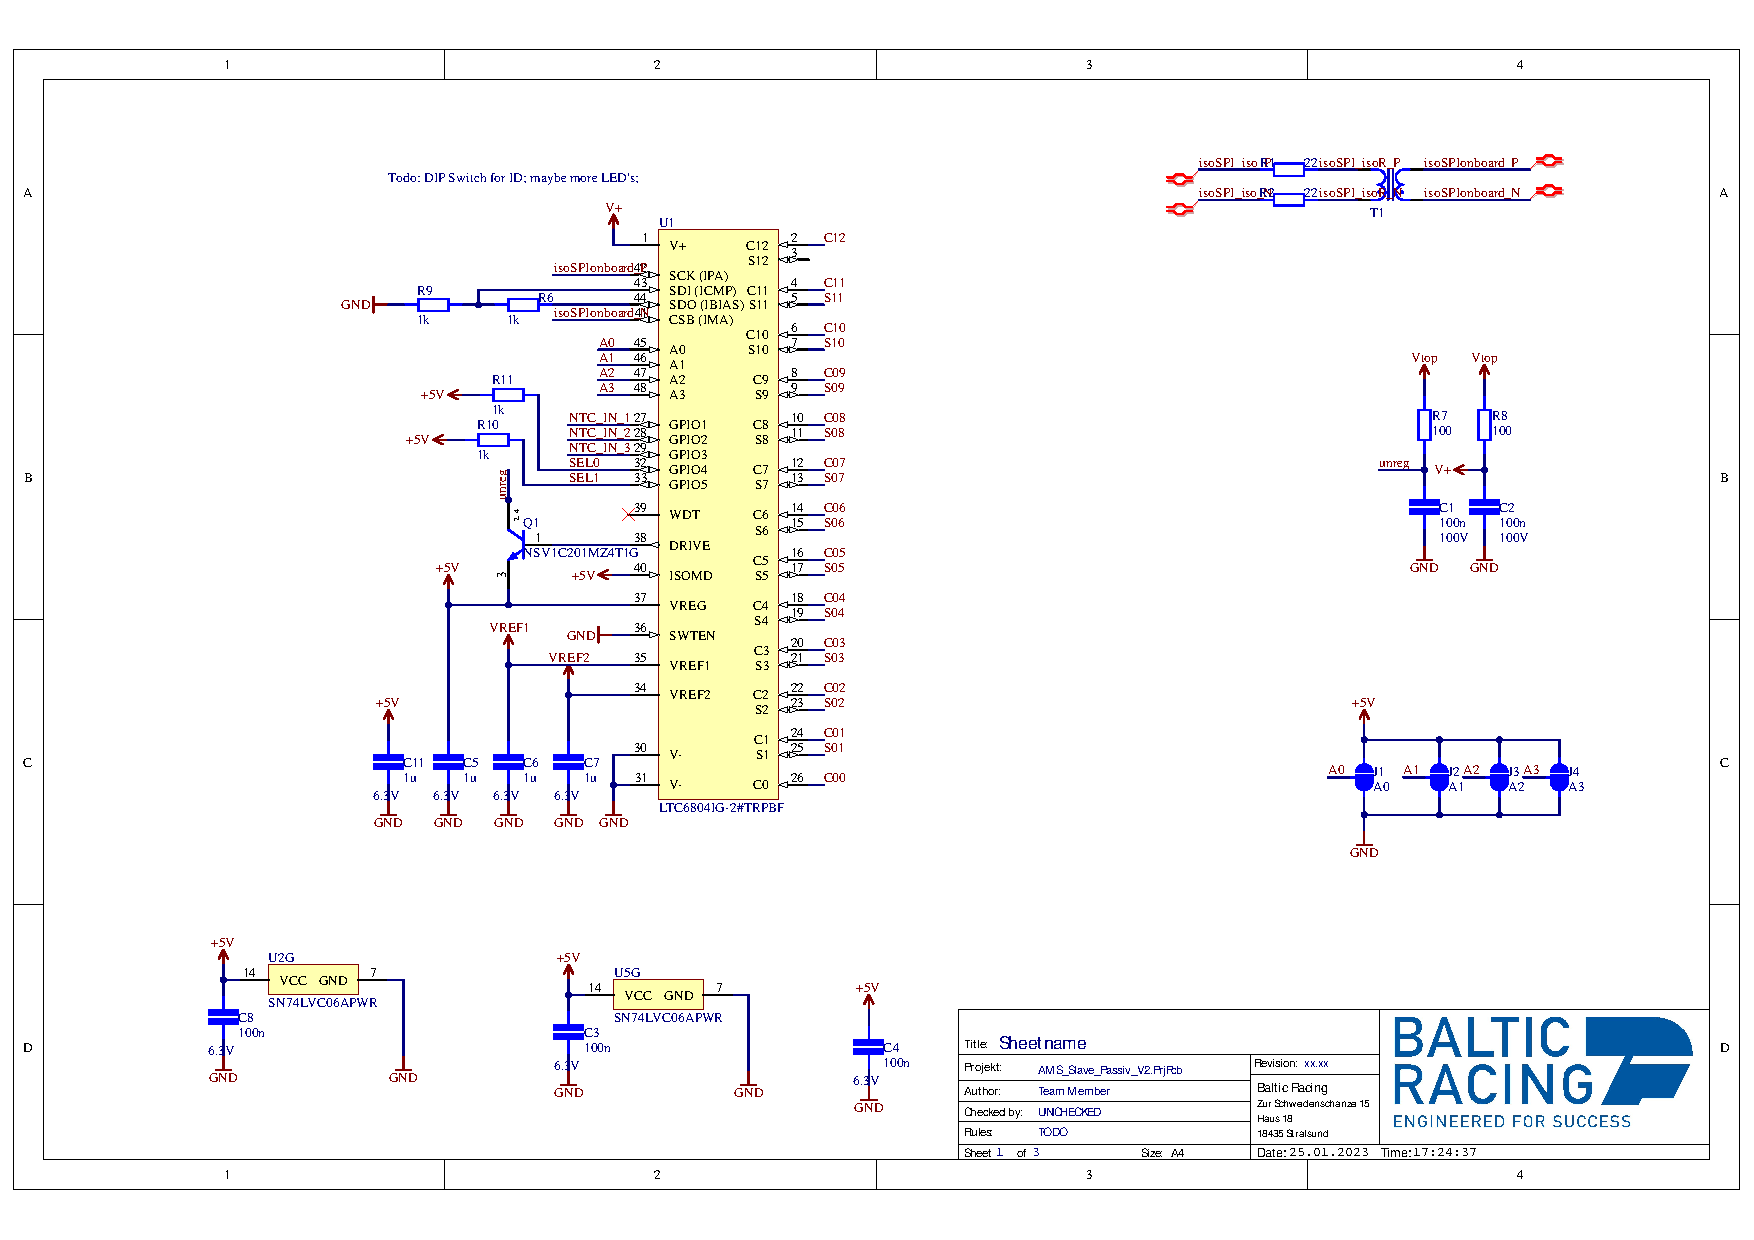
\includepdf[pages=-]{Schaltplaene/AMS_Slave_Passiv_V2.pdf}
\subsection{\ac{BSPD} System}
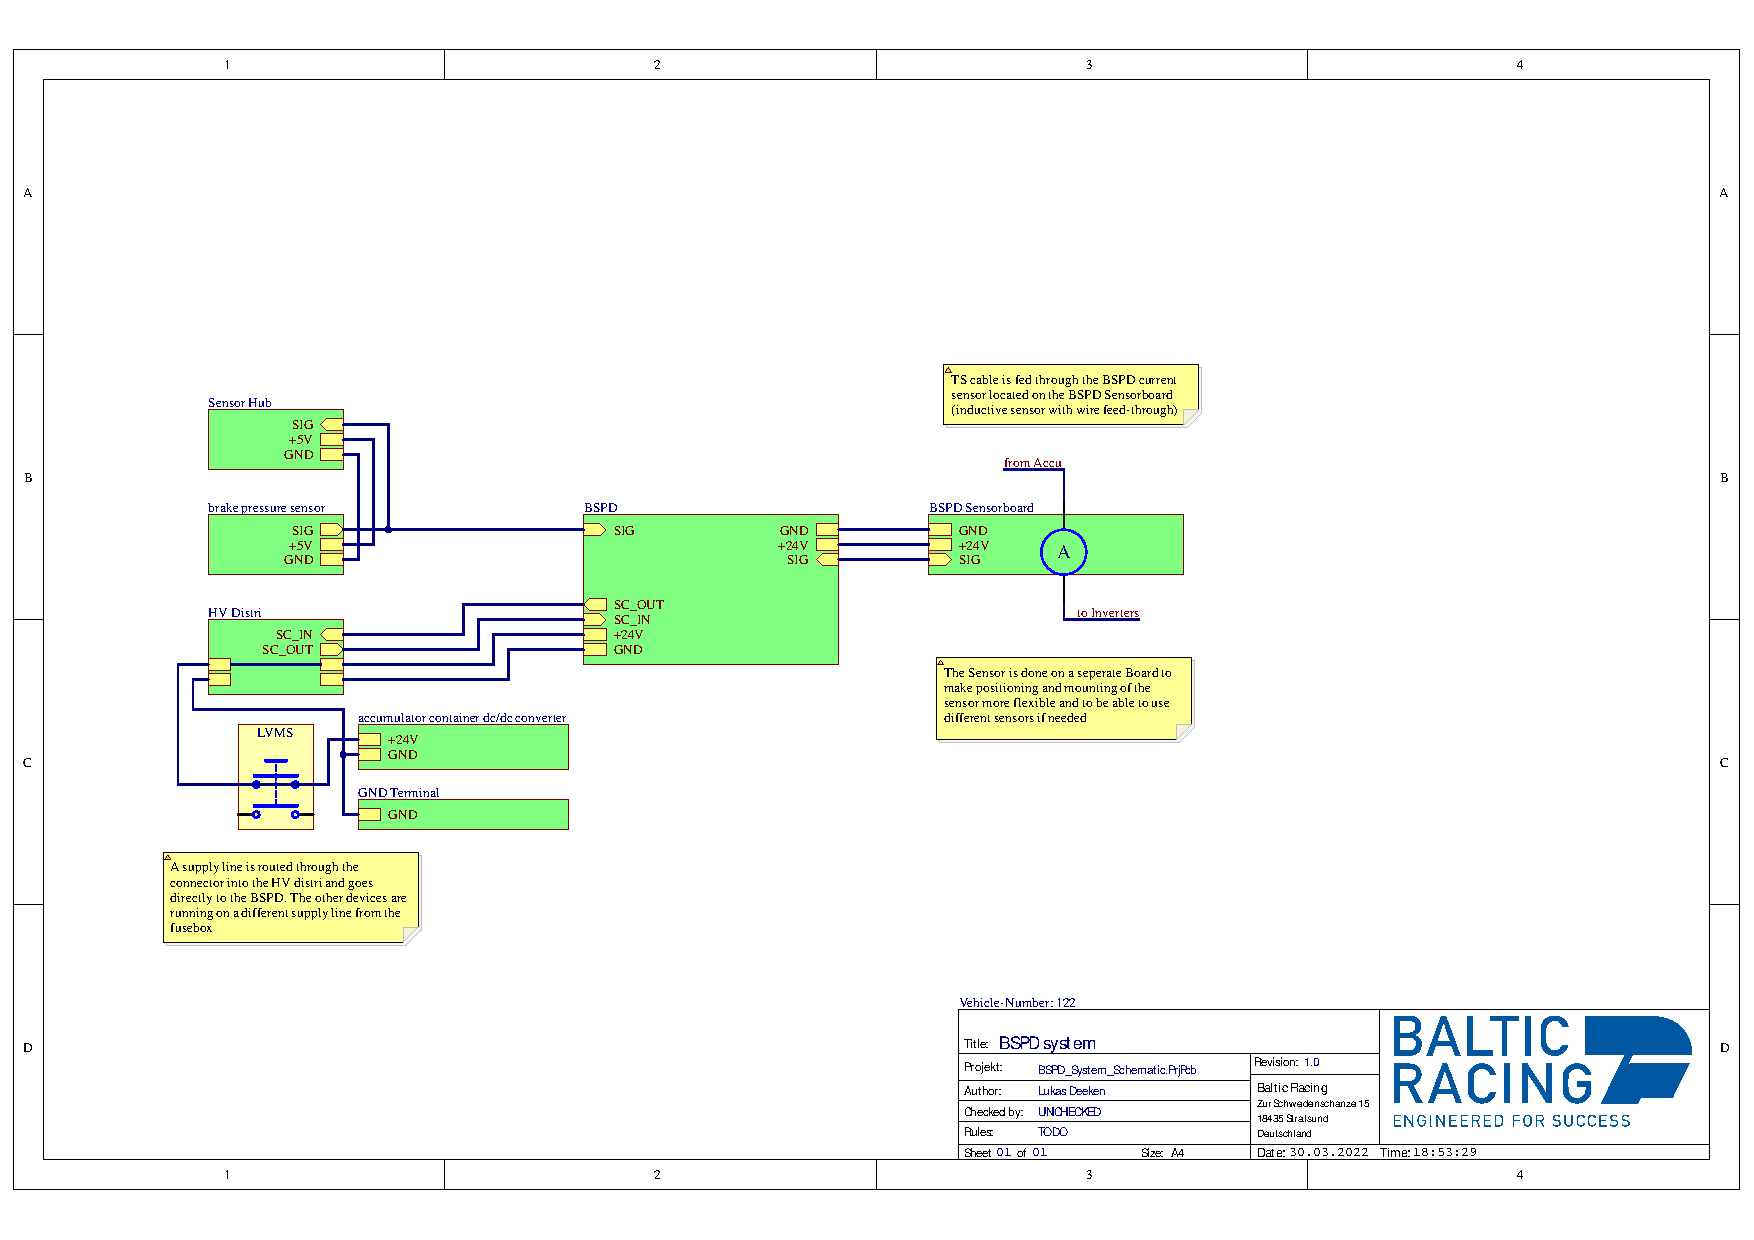
\includepdf[pages=-]{Schaltplaene/BSPD_Schematic_w_System_2.pdf}
\subsection{Chager}
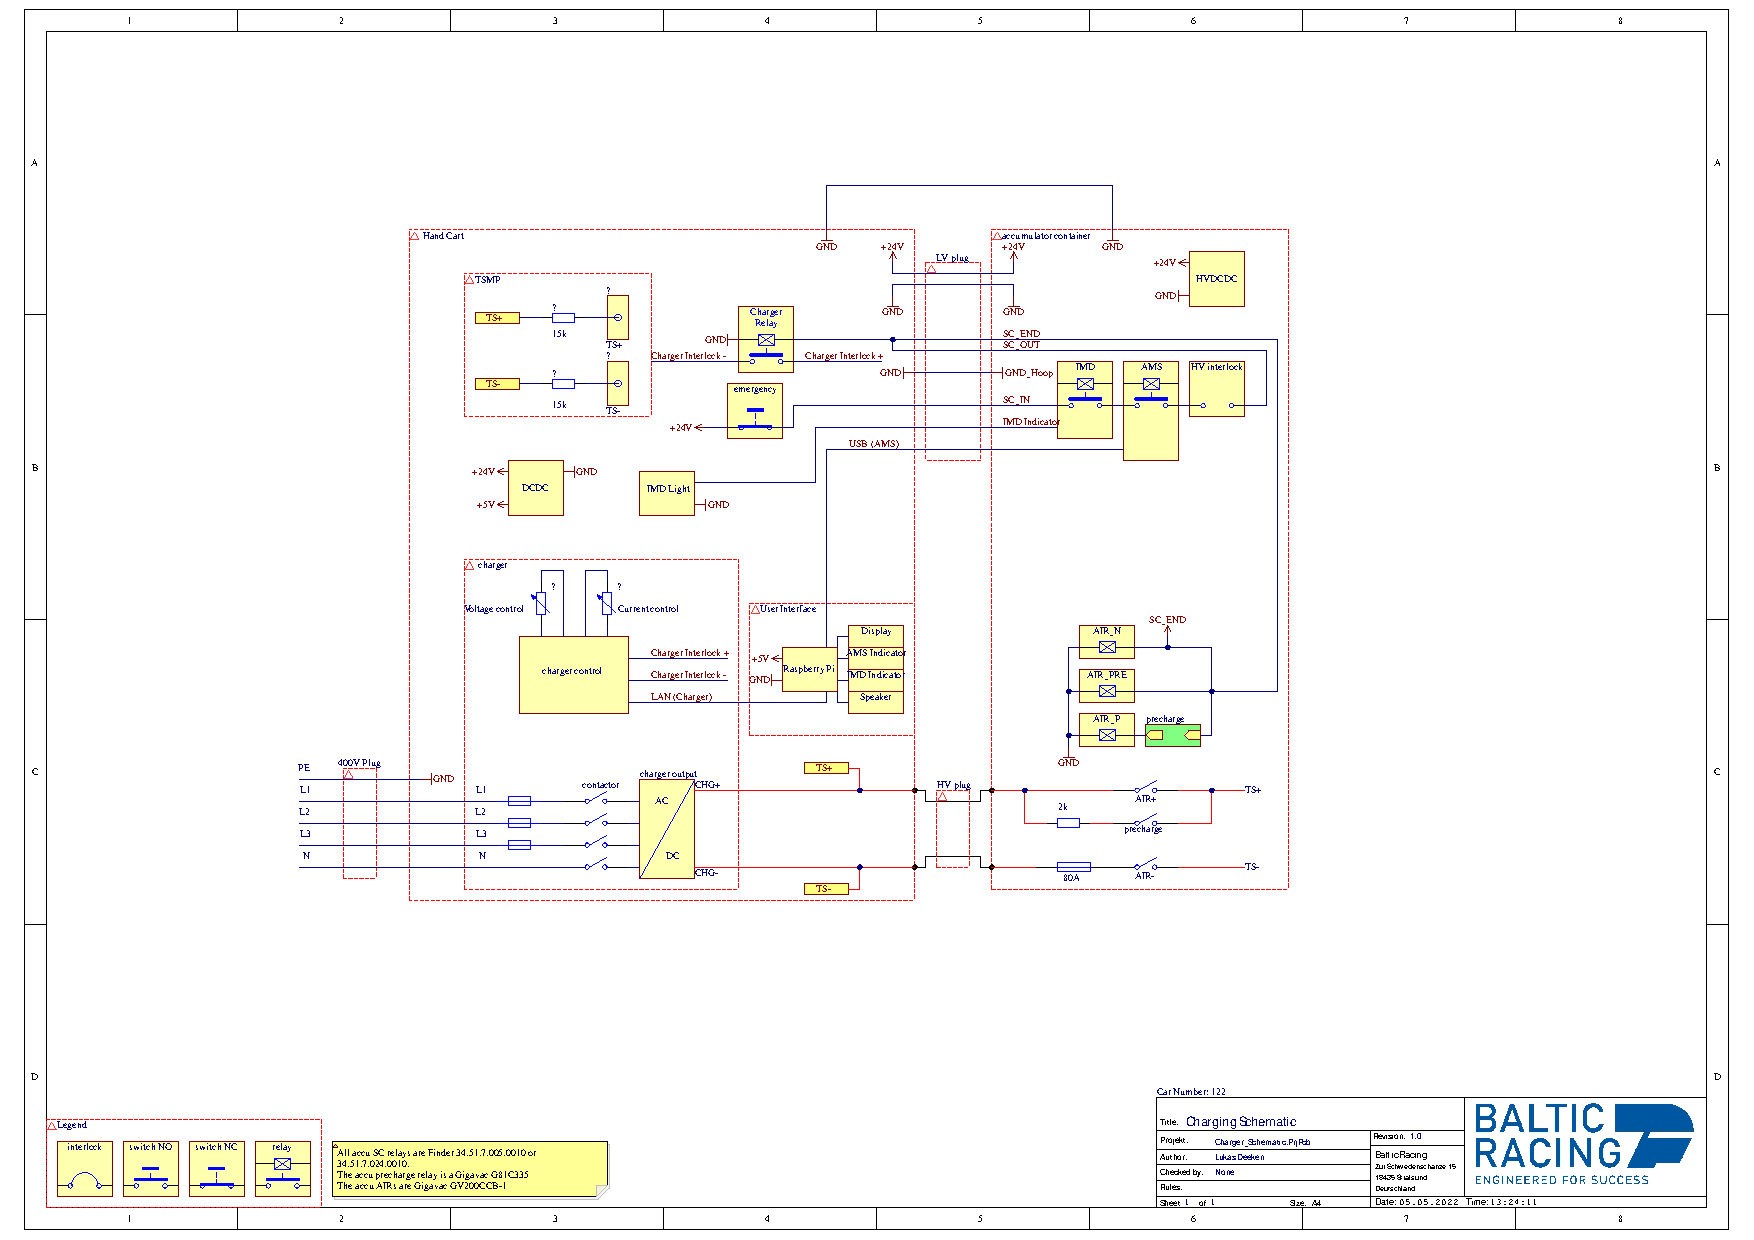
\includepdf[pages=-]{Schaltplaene/Charger_Schematic_V3.pdf}
\subsection{\ac{HV}-DCDC}
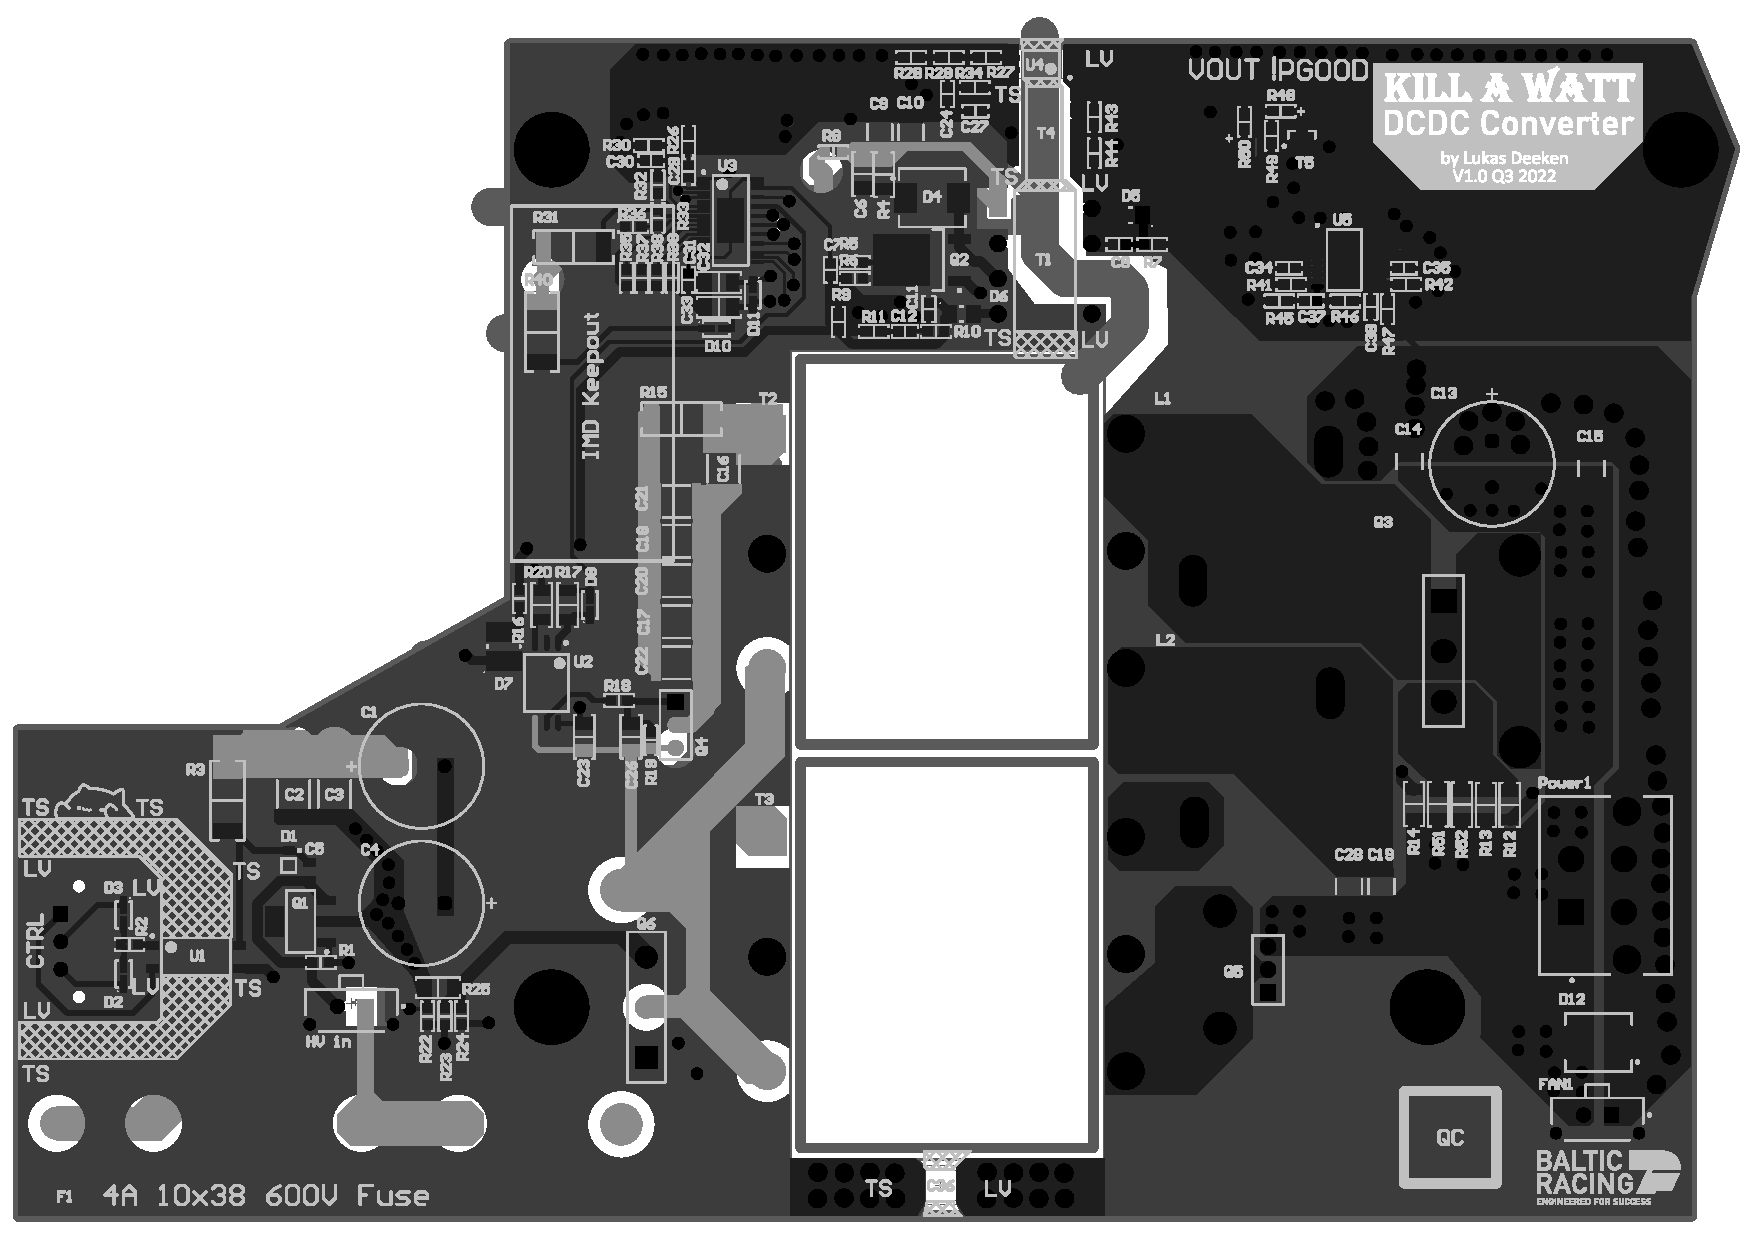
\includepdf[pages=-]{Schaltplaene/HV_DCDC.pdf}
\subsection{HV-Distribution}
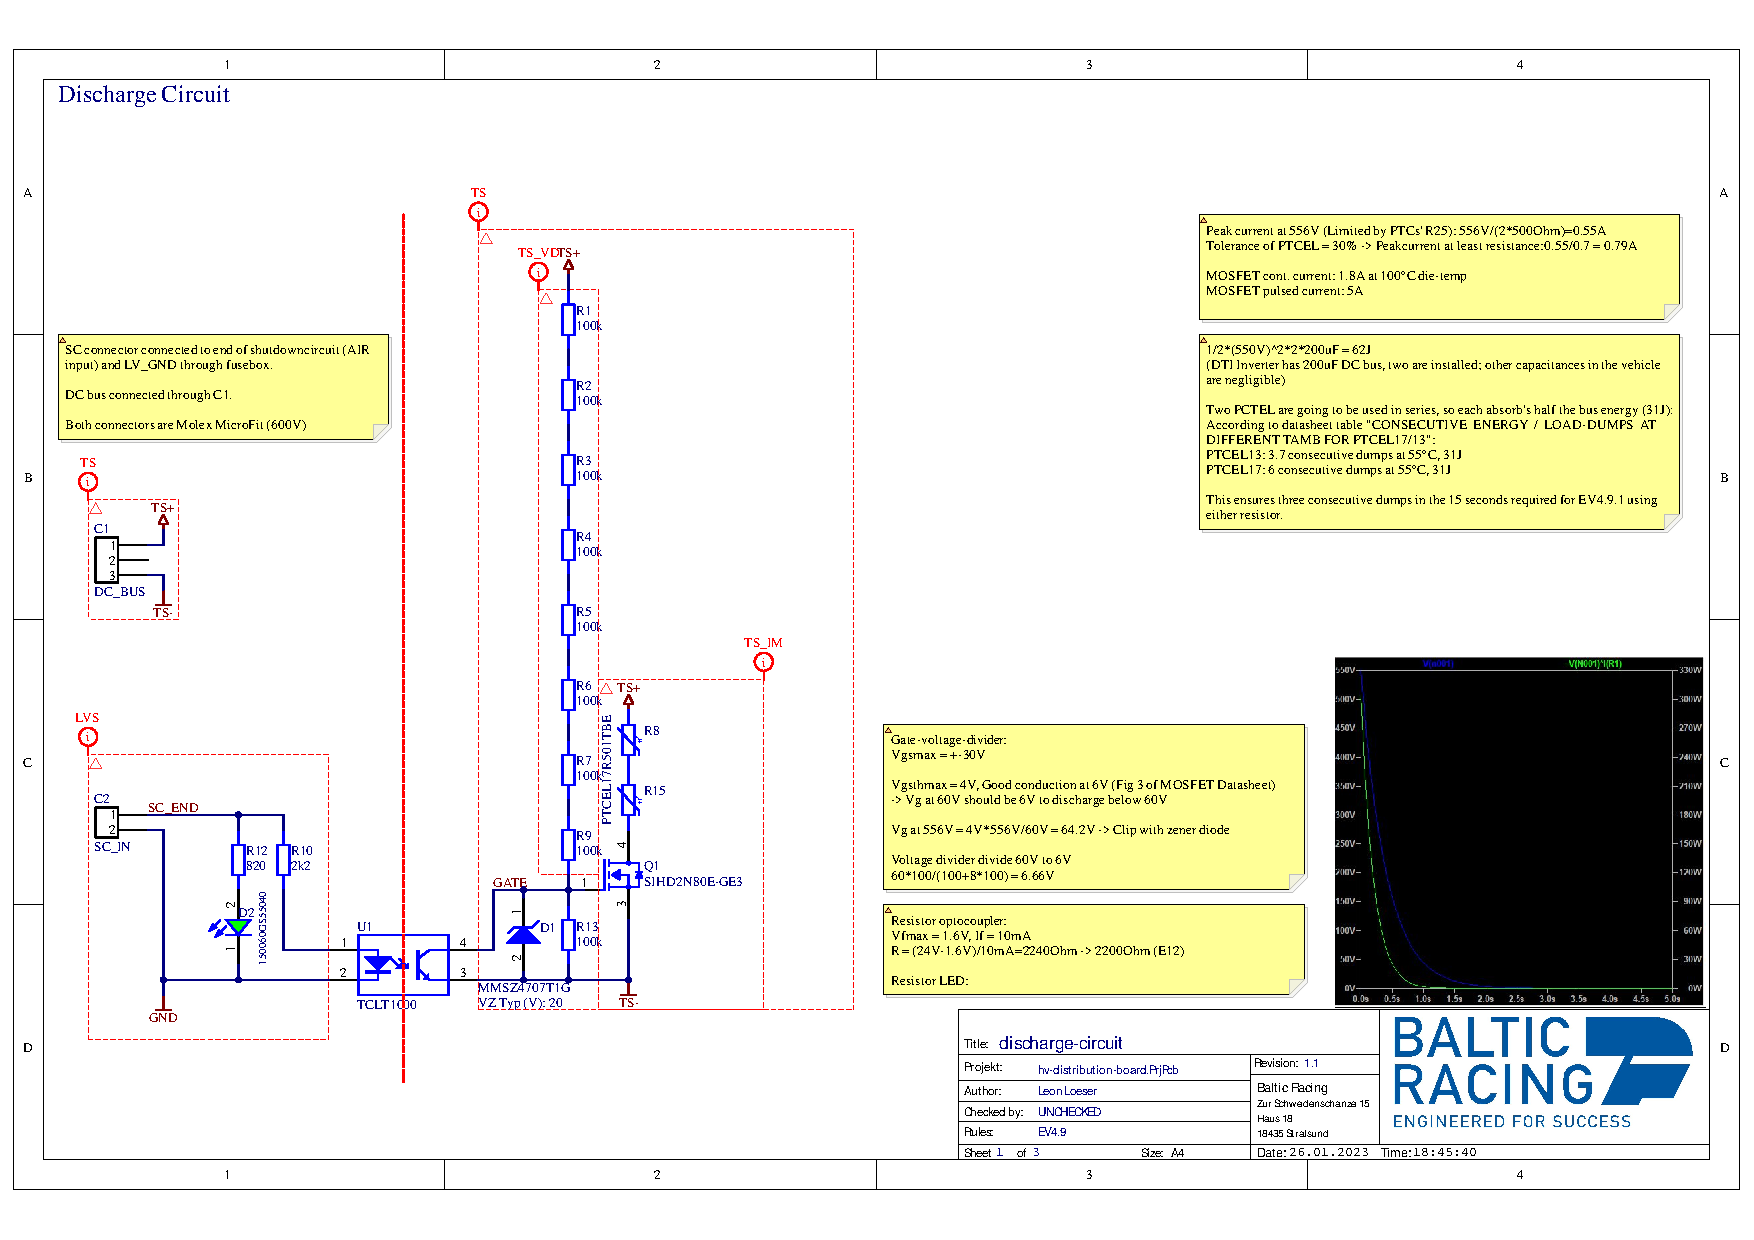
\includepdf[pages=-]{Schaltplaene/hv-distribution-board.pdf}
\subsection{\ac{SDC}}
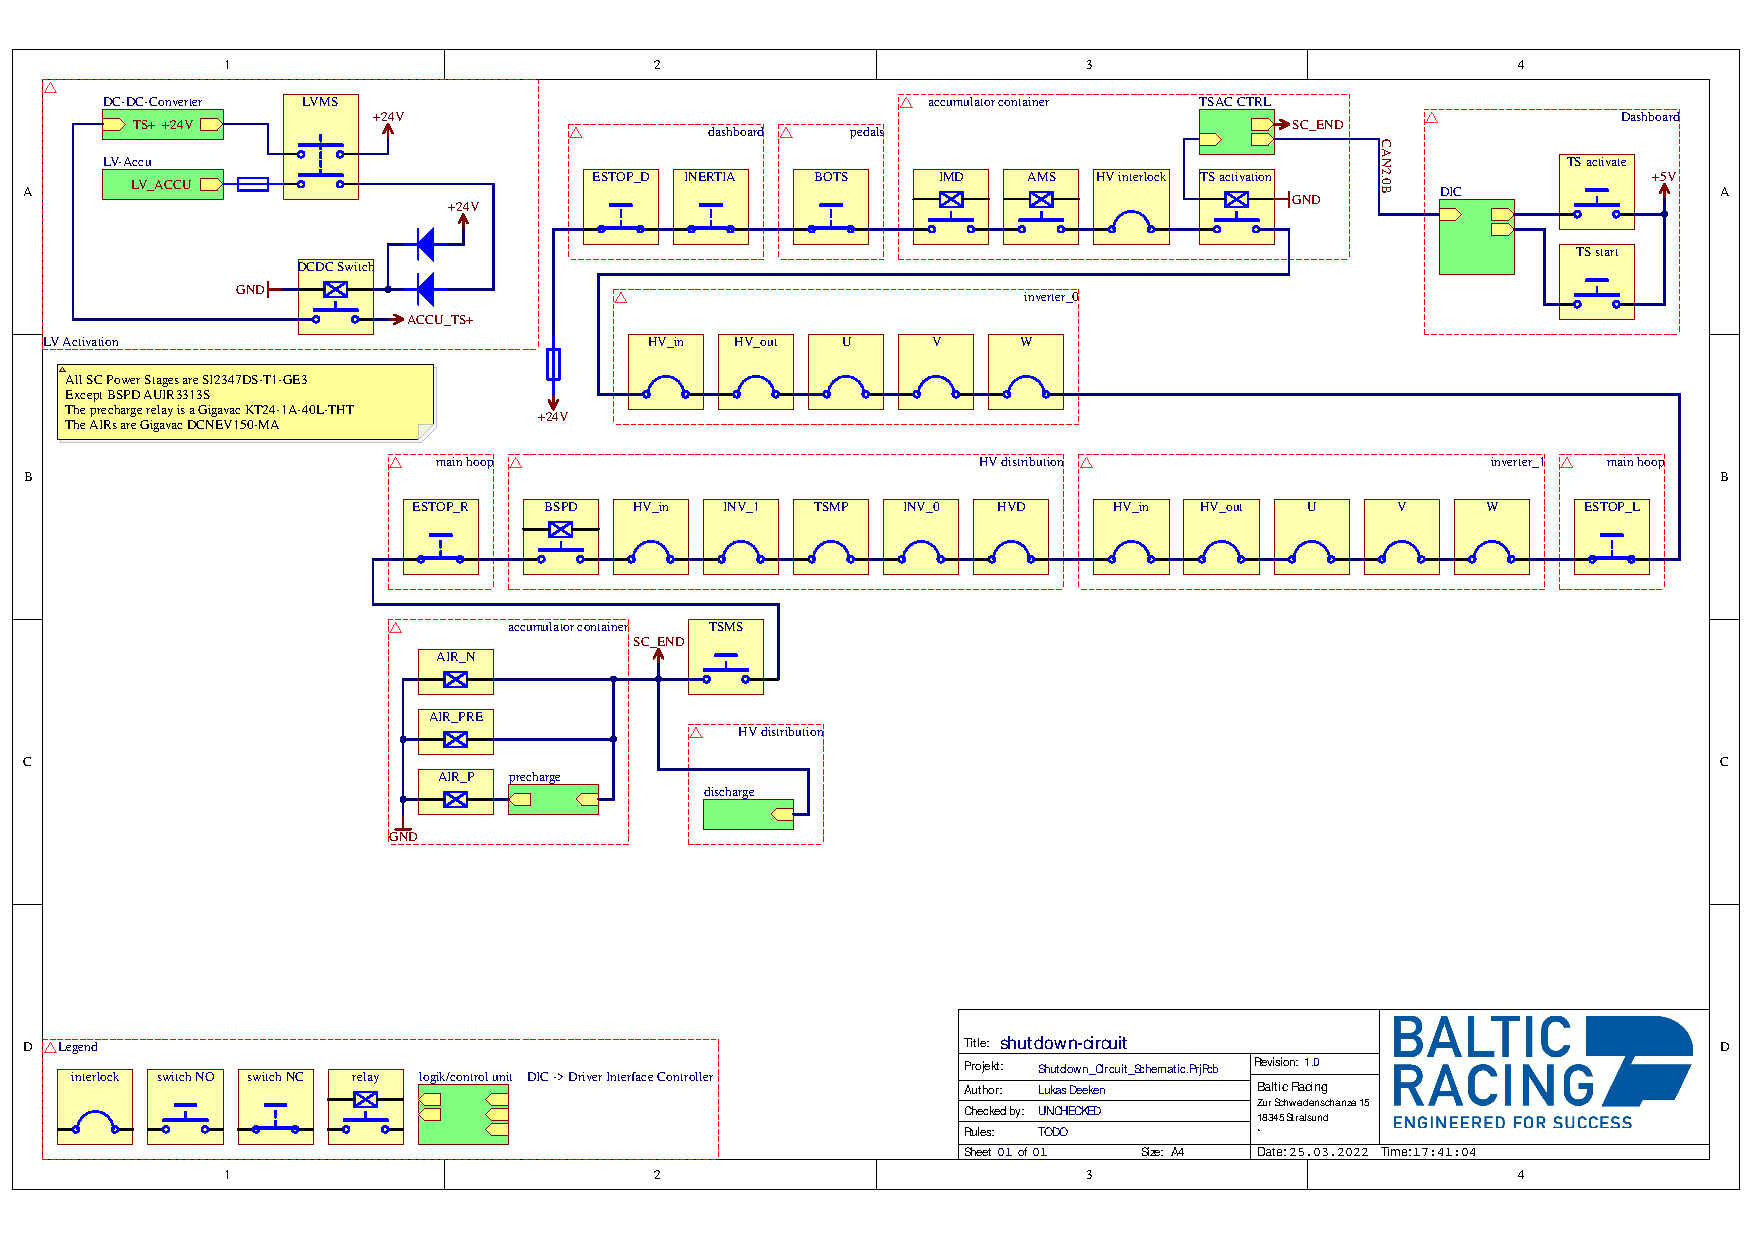
\includepdf[pages=-]{Schaltplaene/Shutdowncircuit.pdf}
\subsection{\ac{TS}-System-Schematic}
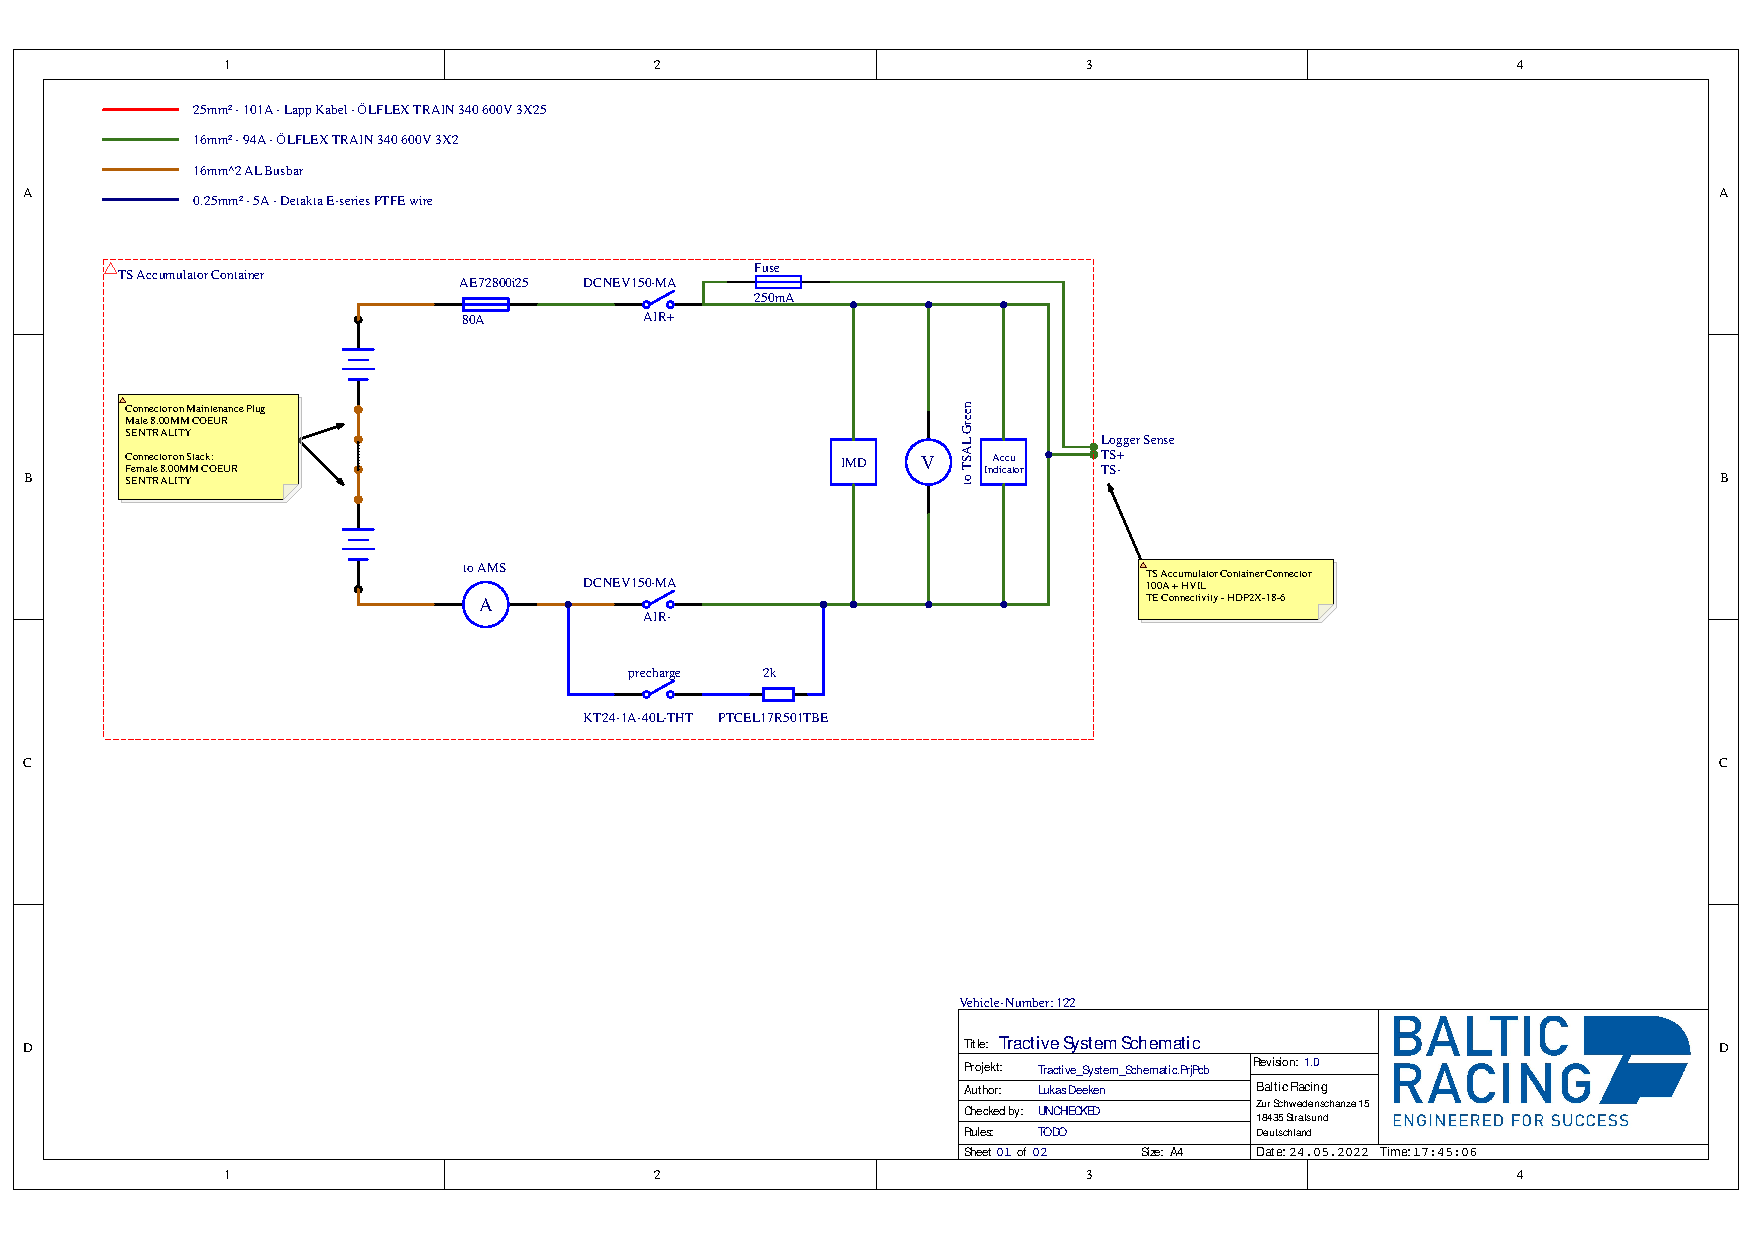
\includepdf[pages=-]{Schaltplaene/Tractive_System_Schematic_V4.pdf}
\subsection{\ac{AMS}-Master}
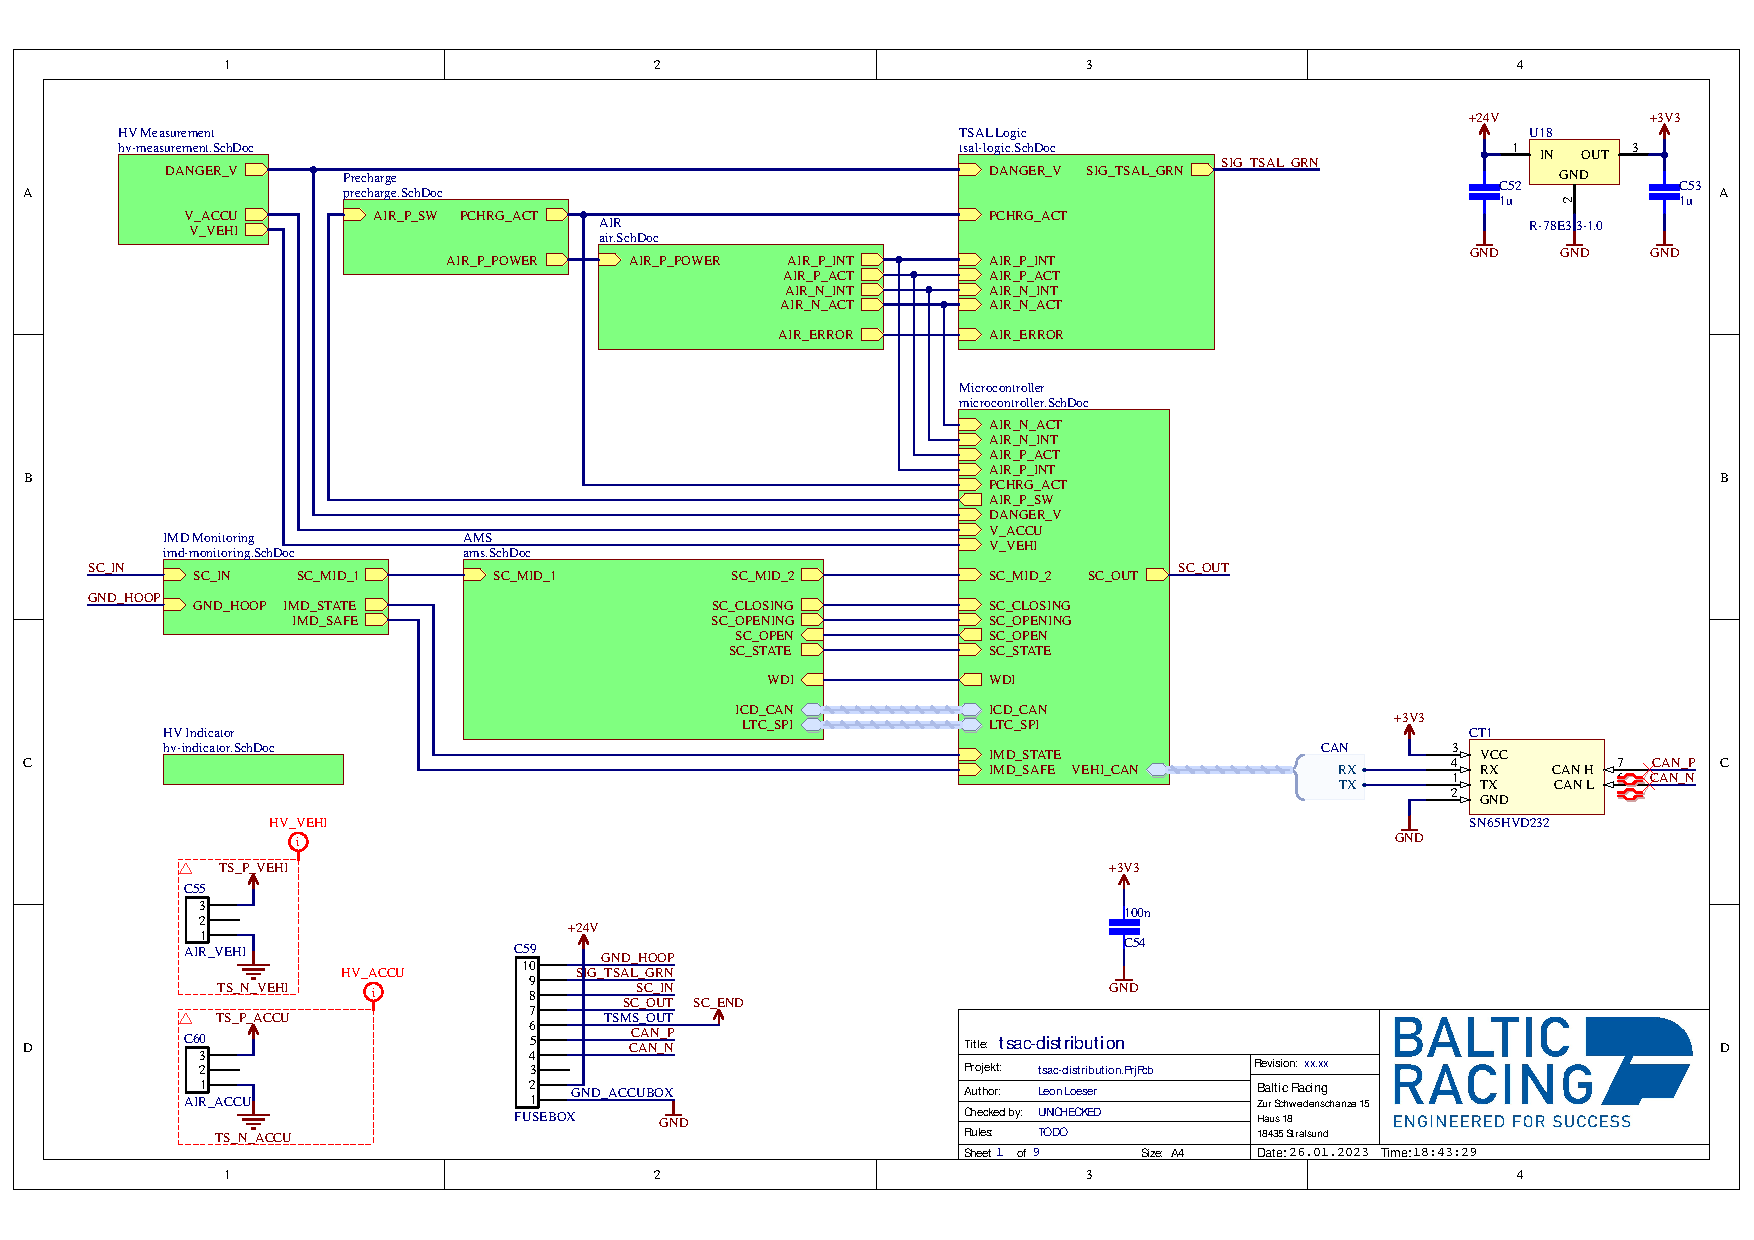
\includepdf[pages=-]{Schaltplaene/tsac-distribution.pdf}
\subsection{\ac{TSAL}}
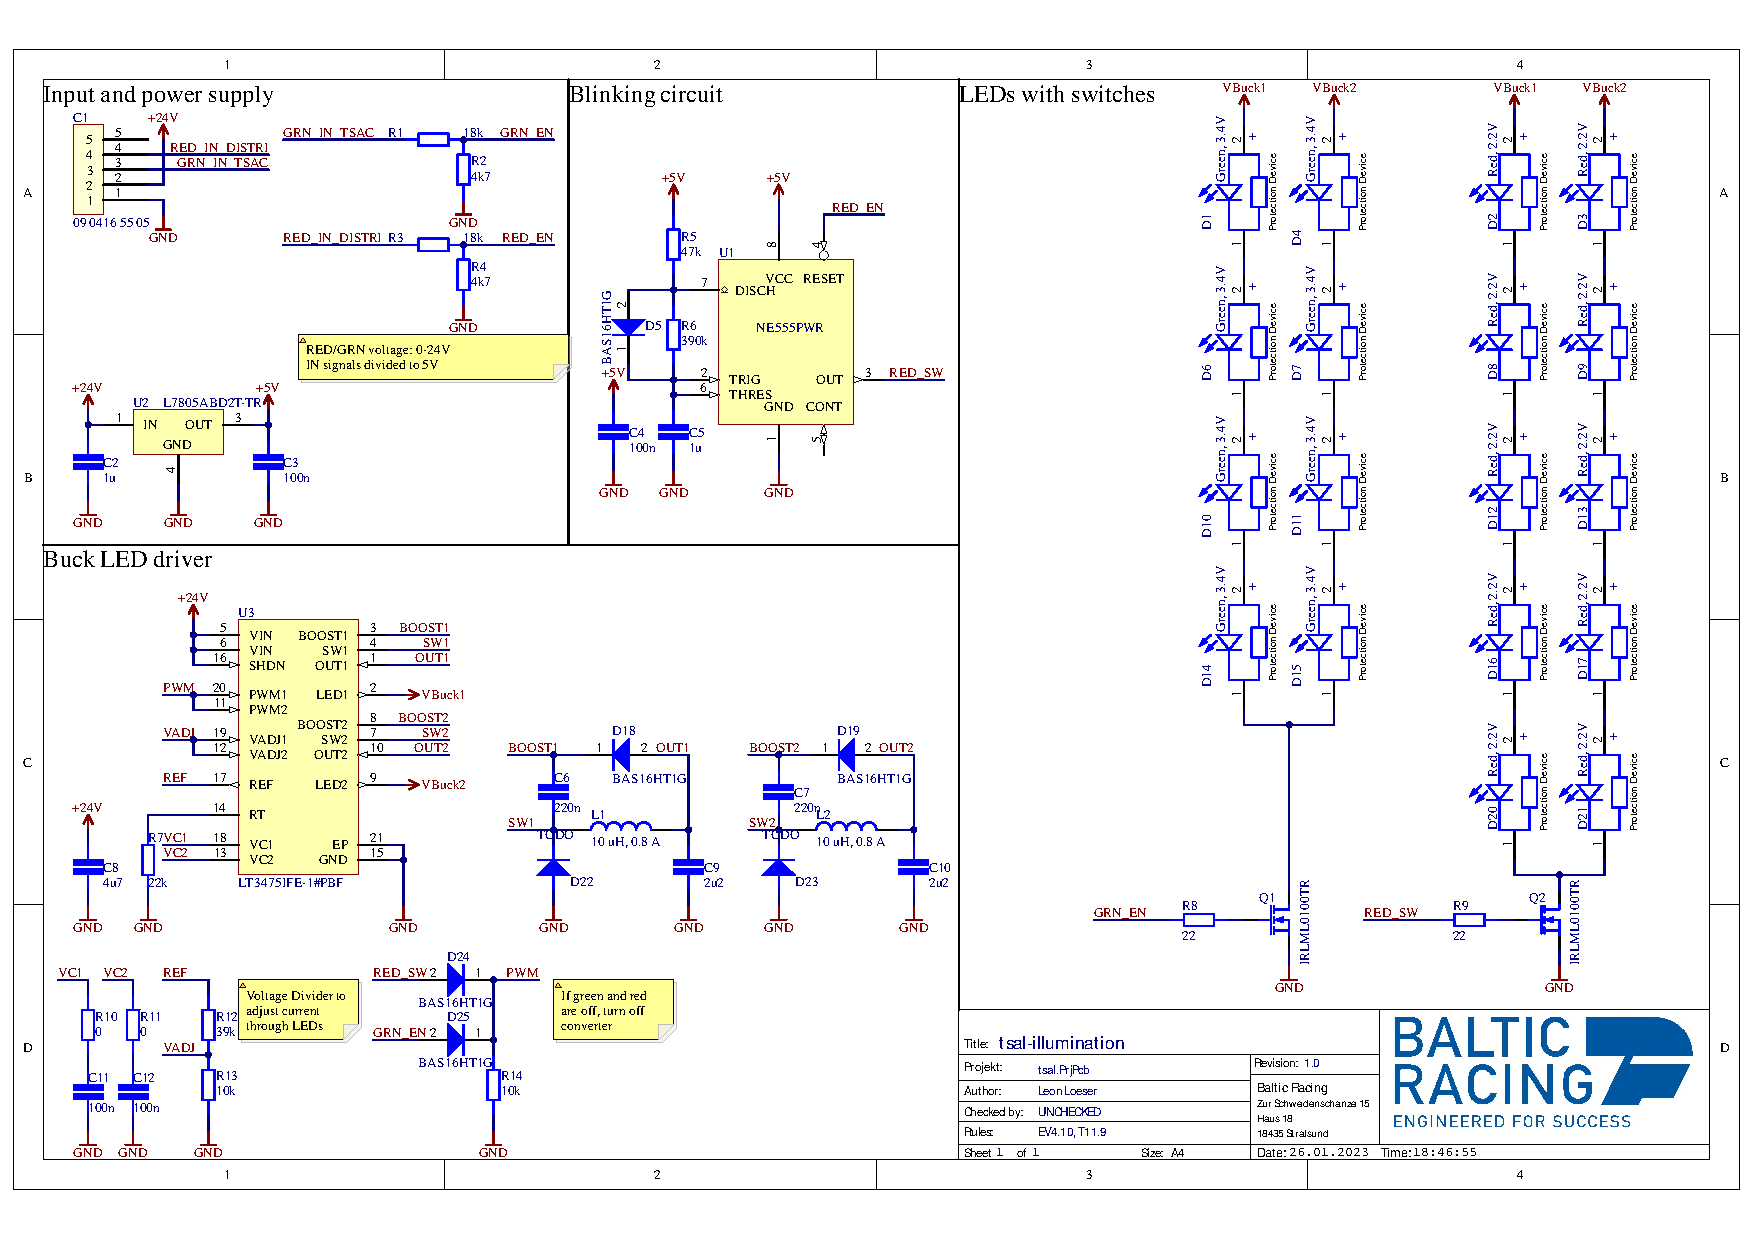
\includepdf[pages=-]{Schaltplaene/tsal.pdf}

	
	\chapter{Zweiter Anhang}
	Beispieltext
	
	%% ++++++++++++++++++++++++++++++++++++++++++++++++++++++++++++
%% Anhang: Beispielkapitel "Programm A"
%% ++++++++++++++++++++++++++++++++++++++++++++++++++++++++++++
%
%  Gerüst:
%  * Version 0.11
%  * Dipl.-Ing. Karsten Renhak, karsten.renhak@tu-ilmenau.de
%  * Fachgebiet Kommunikationsnetze, TU Ilmenau
%
%  Für Hauptseminare, Studienarbeiten, Diplomarbeiten
%
%  Autor           : Max Mustermann
%  Letzte Änderung : 31.12.2011
%

\section{Software A}
Beispieltext

	%% ++++++++++++++++++++++++++++++++++++++++++++++++++++++++++++
%% Anhang: Beispielkapitel "Programm B"
%% ++++++++++++++++++++++++++++++++++++++++++++++++++++++++++++
%
%  Gerüst:
%  * Version 0.11
%  * Dipl.-Ing. Karsten Renhak, karsten.renhak@tu-ilmenau.de
%  * Fachgebiet Kommunikationsnetze, TU Ilmenau
%
%  Für Hauptseminare, Studienarbeiten, Diplomarbeiten
%
%  Autor           : Max Mustermann
%  Letzte Änderung : 31.12.2011
%

\section{Software B}
Beispieltext

		
	% Literaturverzeichnis einbinden
	%% ++++++++++++++++++++++++++++++++++++++++++++++++++++++++++++
%% Anhang: Literaturverzeichnis
%% ++++++++++++++++++++++++++++++++++++++++++++++++++++++++++++
%
%  Gerüst:
%  * Version 0.11
%  * Dipl.-Ing. Karsten Renhak, karsten.renhak@tu-ilmenau.de
%  * Fachgebiet Kommunikationsnetze, TU Ilmenau
%
%  Für Hauptseminare, Studienarbeiten, Diplomarbeiten
%
%  Autor           : Max Mustermann
%  Letzte Änderung : 31.12.2011
%

% Mit dem Befehl \nocite werden auch nicht im Text zitierte
% aus der Literaturdatenbank mit in das Literaturverzeichnis aufgenommen.
% Ein "\nocite{*}" übernimmt ungeprüft die komplette Datenbank.
%\nocite{*}

\cleardoublepage
\ihead[]{Literaturverzeichnis}
\bibliographystyle{alphadin}
\bibliography{literatur} % "literatur.bib" ist hier die einzige Literaturdatenbank.
% Alternativ: Mehrere Datenbanken verwenden, falls eine
% oder mehrere umfangreiche Sammlungen exisitieren:
%\bibliography{literatur_buecher,literatur_weblinks}

	
\end{document}

